~\label{chap:spp}
\begin{chapterabstract}
This chapter introduces an approach to the simultaneous prediction of object shape 
and pose from stereo image pairs. A novel, data driven approach is taken that utilises 
the representational power of Convolutional Neural Networks with the generative power of 
Gaussian Processes.
\end{chapterabstract}
% TODO: extend this abstract.

\section{Introduction}
~\label{sec:spp_introduction}
In the Computer Vision literature, there has been research on the reconstruction of objects
from observed points in a range image, such as those obtained with an RGBD sensor (like 
the Microsoft Kinect). As outlined in Chapter~\ref{chap:probobj}, progress has been made 
on the techniques used, such that globally consistent models of an object of interest can be 
easily obtained.

Though the traditional reconstruction paradigm is suitable for tasks such as 3D data 
collection, it is less applicable in scenarios where full sensor coverage of the object 
of interest is not possible, as outlined in the research problems in Section
~\ref{sec:intro_aims_structure}. When a full view of an object is not available, only a 
partial reconstruction may be built. Data driven, learning based approaches that yield 
reconstructions as predictions from a generative model, however, do not have such a limitation. 
However, for application as a direct replacement for manual reconstruction, pose estimation 
must also be performed.

There has been much progress on learning based methods for both pose estimation and 
shape prediction, as outlined in Section~\ref{sec:lit_review_prediction}. However, much of 
this progress has been on the two problems when decoupled. In this work, an approach is 
proposed to the problem of simultaneous shape and pose prediction. The first 
difference in this work to those outlined in Chapters~\ref{chap:moseg} and~\ref{chap:probobj} 
is the use of stereo RGB frames versus RGBD\@.

The reason for the change of input data format is twofold. First, the use of RGBD is prohibitive 
when considering outdoor environments where lighting conditions may prevent RGBD sensors, such as the 
Microsoft Kinect, from producing a meaningful depth map. Second, the intuition that utilising multiple 
views of an object (from each sensor in the stereo pair) will make the pose estimation more amenable to 
learning based methods, due to the inherent disparity information from the frame pair.

The second major deviation from the contributions of Chapters~\ref{chap:moseg} and~\ref{chap:probobj} 
is the removal of the dependence on temorally consistent input sequences. Rather, in this work 
the proposed system performs shape and pose prediction from an instantaneous
stereo pair, requiring no temporal consistency in both the training and prediction 
phases. As such, there is no iterative solving for shape and pose per frame, rather, the process 
is framed as an instantaneous regression task. However, this work makes use of volumetric
shape representations, as with the other works outlined in Chapters~\ref{chap:moseg} and
~\ref{chap:probobj}.

The approach outlined in this chapter makes use of Siamese~\cite{Bromley1993} 
CNN's and GPLVM's to jointly regress shape and pose given a stereo pair with an object of interest 
present in both frames. The training of the model is unsupervised and requires only a segmentation 
of the object of interest in the input frames to train. The proposed system regresses rotational and 
translational parameters directly from the neural network component, whilst the object shape is 
a draw from a GPLVM\@. The use of a GPLVM for latent space embeddings of 3D shape allows for a simple 
way to learn complex 3D geometrical features, thus simplifying the learning tasks of the neural network. 
In the proposed approach, the neural network component need only learn a mapping from observation to latent 
space, rather than from observation to full geometry for the shape of interest.

The system is trained on an information theoretic loss over a rendering of a predicted 
shape under it's associated predicted pose, with respect to a given detection segmentation. As such, the 
model is trained in a weakly-supervised manner, with neither ground truth shape or pose. Though such an 
approach presents a greater challenge than in the case of known ground truth, it does widen the applicability 
of the approach. In many \textit{real world} scenarios it is not possible to obtain such ground truth data 
without first solving the problem of this work, itself, first.

As outlined previously, the proposed approach differs from that of Chapters~\ref{chap:moseg} and~\ref{chap:probobj} 
in that it is data driven. Rather than instantaneous algorithmic procedures being performed at each frame, the 
result of the input frames is derived from a learnt model. As outlined in Sections~\ref{sec:intro_spp} and
~\ref{sec:intro_aims_structure}, the research interest is in shape and pose prediction for objects in larger scale, 
\textit{real world} environments. As such, the dataset used in this work is the 
\textit{The KITTI Vision Benchmark Suite}~\cite{Geiger2013,Menze2015,Geiger2012}, which consists of a variety of frames 
taken in RGB stereo, from a sensor rigged on top of a car. The dataset is thus suitable to the initial objective 
of real world application.

The remainder of this chapter is structured as follows; Section~\ref{sec:spp_algorithm} introduces the high level 
structure of the proposed model and the structure of it's neural network components. Section~\ref{sec:spp_gplvm} 
introduces and derives the GPLVM that provides a generative model over shape. Following the introduction 
of the GPLVM, Section~\ref{sec:spp_latent_shape_est} outlines the process of extracting a candidate shape for the observed 
object segmentation, from the GPLVM\@. Sections~\ref{sec:spp_pose_estim} and~\ref{sec:spp_rendering} outline the attitude 
representation of pose and shape rendering method used. Though, these are akin to those of Sections
~\ref{subsub:moseg_static_camera_attitude} and~\ref{subsec:moseg_static_rendering}, respectively, the rendering stage is 
modified to introduce the property of differentiability. Sections~\ref{sec:spp_loss} and~\ref{sec:spp_backprop} 
outline the loss function of the model and it's gradient for Backpropagation, respectively. Sections~\ref{sec:spp_qualitative} 
and~\ref{sec:spp_quantitative} provide qualitative and quantitative results on the aforementioned dataset, respectively. 
Finally, Section~\ref{sec:spp_discussion} provides a summary of the approach taken in this work and the preliminary results 
of it's use.

\section{Algorithmic Overview}
~\label{sec:spp_algorithm}
The proposed model takes as input an RGB stereo pair with the object of interest within the 
view frustrum of both frames. From this stereo pair, a ResNet~\cite{He2015} extracts feature descriptors 
which are used to regress a latent space point for shape, and six \( \mathbb{SE}(3) \) pose parameters, forming 
a Lie Algebra. The generated shape for the proposal latent space point is drawn from the distribution of 
the Gaussian Process (GP) prior conditioned on the latent space point. The form of the pose is the Lie 
Group mapping of the parameters, as given in Sections~\ref{subsub:moseg_static_camera_attitude} 
and~\ref{subsec:probobj_analytic_alignment_map}. 

The goodness of fit of the regressed shape and pose is quantified by by rendering the generated shape 
under the predicted pose and computing an information theoretic loss between the image statistics of 
the rendered region vs the initial segmentation region. To maintain continuity, the rendering operation is 
formulated in a differentiable manner. As there is often no ground truth pose and shape for \textit{real world} 
data, training is performed in a weakly-supervised manner against a segmentation of the object of interest.

\subsection{Model Architecture}
~\label{subsec:spp_network_architecture}
The model of the proposed approach is of a Siamese topology, where for a given stereo 
pair, each of the left and right frames are passed to a separate network. From end to 
end, the model contains for each of the Siamese networks a ResNet-101~\cite{He2015}, 
Linear Layers, Batch Normalisation Layers, Nonlinear Activations, a mapping from Lie Algebra to 
Lie Group (for pose), a GPLVM followed by an Inverse Discrete Cosine Transform (IDCT), a Raycaster and 
an information theoretic loss. 

The purpose of the ResNet-50 components is to extract pertinent features from the stereo 
pair that are descriptive of the the object of interest in relation to the scene. For each 
of the networks, the output of the ResNet-101 network is fed into two subnetworks consisting 
of linear transforms and nonlinear activations. The purpose of these subnetworks is to regress 
a latent space point for object shape, and a 6DoF pose parameter vector for the object pose. 
Following these two subnetworks is the aforementioned GPLVM and Lie Algebra mapping. The 
GPLVM generates a posterior mean over shape for a given latent space point, whilst the 
Lie Algebra mapping generates an \( \mathbb{SE}(3) \) transform. 

The IDCT decompresses the posterior mean output of the GPLVM to generate a valid SDF\@. Both the 
resultant SDF and \( \mathbb{SE}(3) \) transform are passed to the Raycasting module, which generates 
a rendering for the candidate shape and pose. Finally, this rendering with the initial detection is passed 
to the loss layer which computes appearance statistics for the detection region and the rendering 
which are used to quantify loss. The topology of the proposed model is outlined in Figure
~\ref{figure:spp_pipeline}.
\begin{landscape}
  \begin{figure}[!htbp]
    \centering
    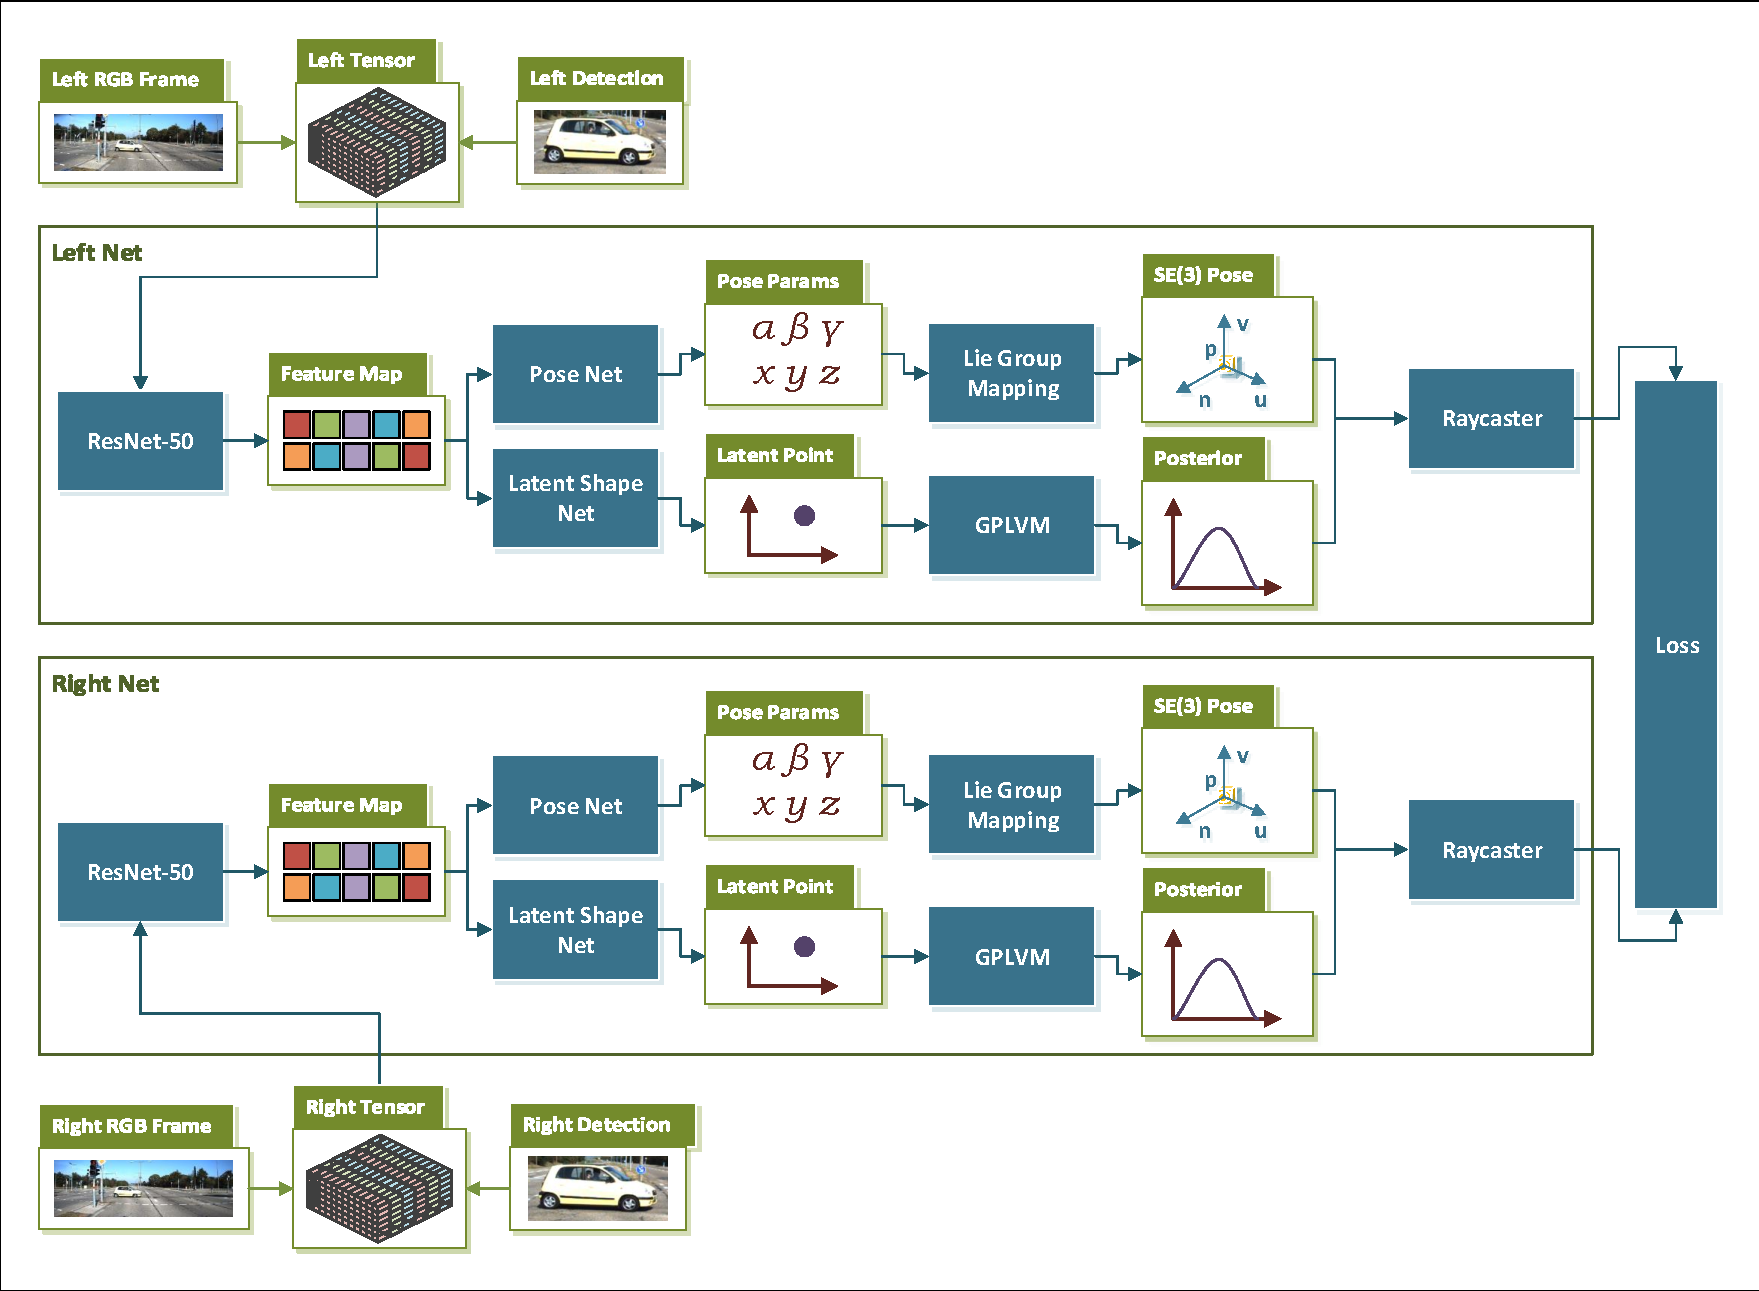
\includegraphics[width=.8\linewidth]{figures/spp/model.pdf}
    \caption[Shape and Pose Prediction Network]{The proposed shape and pose prediction network. 
    Note that the \textit{ResNet-50}, \textit{Shape Net} and \textit{Latent Net} components have 
    shared parameters.}
~\label{figure:spp_pipeline}
  \end{figure}
\end{landscape}

\subsection{Neural Network Architecture}
~\label{subsec:spp_neural_architecture}
The ResNet architecture, introduced by \textit{He at al}~\cite{He2015}, is designed to overcome the 
convergence challenges of very ``deep'' neural network models. The central reformulation in the 
Residual Network model is the notion that layers learn \textit{residual functions} with respect to 
their inputs. Instead of a layer learning a mapping \( \mathcal{H}(\bm{x}) \) of it's input \( \bm{x} \), 
it learns a \textit{residual} mapping, as given in Equation~\ref{eqn:resnet}.
\begin{align}
~\label{eqn:resnet}
  \mathcal{F}(\bm{x}) ={}& \mathcal{H}(\bm{x}) - \bm{x}\\
  \mathcal{F}(\bm{x}) + \bm{x} ={}& \mathcal{H}(\bm{x})
\end{align}

The formulation of Equation~\ref{eqn:resnet} is depicted in Figure~\ref{figure:resnet_block}.
\begin{figure}[!htbp]
  \centering
  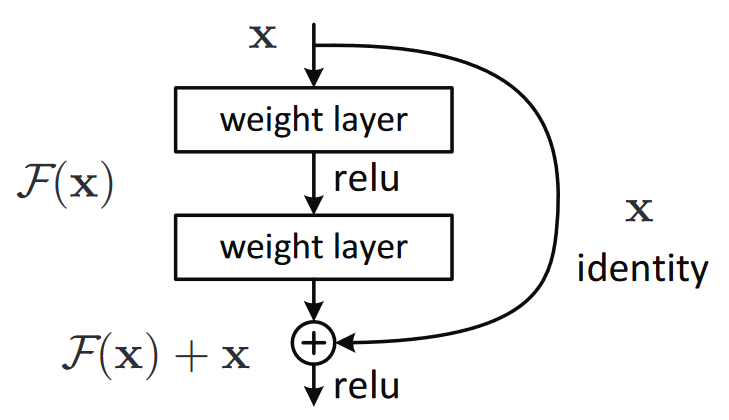
\includegraphics[width=.6\linewidth]{figures/spp/residual_block_he.png}
  \caption[ResNet Block]{The central building block of the ResNet architecture.\footnotemark}
~\label{figure:resnet_block}
\end{figure}
~\footnotetext{Image copyright: \textit{He et al}~\cite{He2015}.}

% TODO: Reorder this; goes from high level intro to GP's... bit heavy 
\section{Gaussian Process Latent Variable Model}
~\label{sec:spp_gplvm}
The use of a GPLVM for the embedding of 3D shape is motivated by the assumption that for a 
given category of object, cars for example, there is enough shared geometric structure that 
a comprehensive generative model may be formed. In the linear case, the GPLVM is equivalent 
to a probabilistic formulation of Principal Component Analysis (PCA), where a linear mapping 
from observed to hidden, latent space is derived. 

Under a Bayesian formulation, the often intractable latent variables pertaining to the linear 
mapping may be marginalised such that the latent embedding itself may be optimised directly. The 
given framework allows for complex, nonlinear embeddings to be learnt via the use kernel functions, 
though the optimisation in this case is often non-convex and highly nonlinear.

A Gaussian Process may be viewed as a prior distribution over continuous functions. The posterior 
may be obtained by conditioning on observed data, to obtain a function estimate for each data point.
A visual example of a GP is given in Figure~\ref{figure:gp_func_dist}.
\begin{figure}[!htbp]
  \centering
  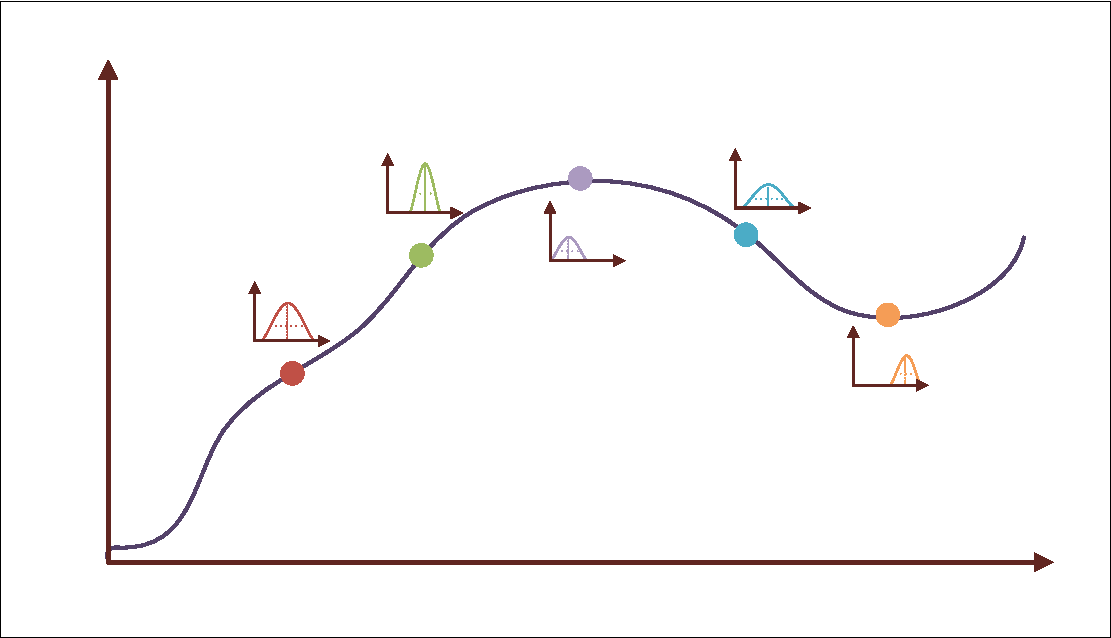
\includegraphics[width=\linewidth]{figures/spp/gp.pdf}
  \caption[GP as a Distribution Over Functions]{For each point along \( x \), 
  a function \( \bm{f} \sim \mathcal{GP}(\bm{\mu}, \bm{\Sigma}) \) drawn from a Gaussian Process 
  \( \mathcal{GP} \) is evaluated at \( x \).}
~\label{figure:gp_func_dist}
\end{figure}

\subsection{Gaussian Process Marginal Likelihood}
~\label{subsec:spp_gp_marginal_likelihood}
The first step is to define a Latent Variable Model of the form given in Equation~\ref{eqn:spp_gp_lvm}.
\begin{equation}
  \label{eqn:spp_gp_lvm}
  P(\bm{Y} \given \bm{X}, \bm{W}, \beta) = P(\bm{Y} \given \bm{WX}^{T}, \beta^{-1}\bm{I})
\end{equation}
In Equation~\ref{eqn:spp_gp_lvm} the observed data \(\bm{Y} \in \mathbb{R}^{N \times D}\) 
is mapped to a lower dimensionality manifold \(\bm{X} \in \mathbb{R}^{N \times P}\), by parameters 
\(\bm{W} \in \mathbb{R}^{P \times D}\) and variance \( \beta \). In Equation~\ref{eqn:spp_gp_lvm}, 
the latent variable model \( P(\bm{Y} \given \bm{X}, \bm{W}, \beta) \) provides a linear mapping 
defined by the aforementioned latent variables \( \bm{W} \). As \( \bm{W} \) is unobservable and 
thus not directly tractable, it may be analytically marginalised out, given a suitable likelihood 
and prior.

The marginal likelihood of \(\bm{X}\) is of the form outlined in Equation~\ref{eqn:spp_gp_marginal}.
\begin{equation}
  \label{eqn:spp_gp_marginal}
  P(\bm{Y} \given \bm{X}, \beta) = \int P(\bm{Y} \given \bm{X}, \bm{W}, \beta) P(\bm{W}) \intd{\bm{W}}
\end{equation}
In Equation~\ref{eqn:spp_gp_marginal}, \( P(\bm{Y} \given \bm{X}, \bm{W}, \beta) \) is of 
a multivariate Gaussian form and \(P(\bm{W})\) is a multivariate Gaussian conjugate prior of the 
form \(\mathcal{N}(\bm{W} \given \bm{0}, \bm{I})\).

To find the marginal distribution outlined in Equation~\ref{eqn:spp_gp_marginal}, it's form may 
first be simplified as follows in Equation~\ref{eqn:spp_gp_marginal_simplify}.
\begin{align}
  \label{eqn:spp_gp_marginal_simplify}
  % Line 1.
  P(\bm{Y} \given \bm{X}, \beta) ={}& \int \mathcal{N}(\bm{Y} \given \bm{WX}^{T}, \beta^{-1}\bm{I})
  \mathcal{N}(\bm{W} \given \bm{0}, \bm{I}) \intd{\bm{W}} \\
  % Line 2.
  ={}& \int \frac{1}{\sqrt{\left|2\pi\beta^{-1}\bm{I}\right|}} e^{ 
    -\frac{\beta}{2} {\big( \bm{Y} - \bm{WX} \big)}^{T} \big( \bm{Y} - \bm{WX} \big) 
  }
  \frac{1}{\sqrt{\left|2\pi\bm{I}\right|}} e^{ 
    -\frac{1}{2} \bm{W}^{T}\bm{W}} \intd{\bm{W}} \\
  % Line 3.
  ={}& \frac{1}{\sqrt{\left|2\pi\beta^{-1}\bm{I}\right|}} \frac{1}{\sqrt{\left|2\pi\bm{I}\right|}} 
  \int e^{
    -\frac{\beta}{2} {\big( \bm{Y} - \bm{WX} \big)}^{T} \big( \bm{Y} - \bm{WX} \big) 
    -\frac{1}{2} \bm{W}^{T}\bm{W}} \intd{\bm{W}} \\
  % Line 4.
  \propto& \int e^{
    -\frac{\beta}{2} {\big( \bm{Y} - \bm{WX} \big)}^{T} \big( \bm{Y} - \bm{WX} \big) 
    -\frac{1}{2} \bm{W}^{T}\bm{W}} \intd{\bm{W}} \\
  % Line 5.
  \propto& \int e^{ 
  -\frac{1}{2} \Big[
    \beta {\big( \bm{Y} - \bm{X}^{T}\bm{W} \big)}^{T} \big( \bm{Y} - \bm{X}^{T}\bm{W} \big) 
    + \bm{W}^{T}\bm{W}
  \Big]} \intd{\bm{W}} \\
  % Line 6.
  \propto& e^{ -\frac{\beta}{2} \bm{Y}^{T}\bm{Y}} 
  \int e^{
  -\frac{1}{2} \Big[
    -\beta \big( \bm{Y}^{T}\bm{X}^{T}\bm{W} \big) 
    -\beta {\big( \bm{W}^{T}\bm{XY} \big)}^{T}
    +\beta \bm{W}^{T}\bm{XX}^{T}\bm{W}
    + \bm{W}^{T}\bm{W}\Big]} \intd{\bm{W}} \\
  % Line 7.
  \propto& e^{-\frac{\beta}{2} \bm{Y}^{T}\bm{Y}} 
  \int e^{
  -\frac{1}{2} \Big[
    -2\beta \bm{Y}^{T}\bm{X}^{T}\bm{W}
    +\beta \bm{W}^{T}\bm{XX}^{T}\bm{W}
    + \bm{W}^{T}\bm{W}
  \Big]} \intd{\bm{W}} \\
  % Line 7.
  \propto& e^{-\frac{\beta}{2} \bm{Y}^{T}\bm{Y}} 
  \int e^{
  -\frac{1}{2} \Big[
    \bm{W}^{T} \big( \beta \bm{XX}^{T} + \bm{I} \big) \bm{W}
    -2\beta \bm{Y}^{T}\bm{X}^{T}\bm{W}
  \Big]} \intd{\bm{W}}
\end{align}

To make the integral over \(\bm{W}\) tractable in Equation~\ref{eqn:spp_gp_marginal_simplify}, 
the distribution \(P(\bm{Y} \given \bm{X}, \beta)\) must be a Gaussian; an exponential 
of a quadratic form. Completing the square in \(\bm{W}\) allows the marginal to be expressed 
in such a form. First, a change of variables is made, as in Equation~\ref{eqn:spp_gp_marginal_change}.
\begin{align}
  \label{eqn:spp_gp_marginal_change}
  \bm{A} ={}& \beta \bm{XX}^{T} + \bm{I}\\
  \bm{b} ={}& \beta \bm{Y}^{T} \bm{X}^{T}
\end{align}

The procedure to integrate over \( \bm{W} \) and transform \( P(\bm{Y} \given \bm{X}, \beta) \) 
into a valid multivariate Gaussian form is as follows in Equation~\ref{eqn:spp_gp_complete}.
\begin{align}
  \label{eqn:spp_gp_complete}
  % Line 1.
  P(\bm{Y} \given \bm{X}, \beta) \propto{}& e^{-\frac{\beta}{2}\bm{Y}^{T}\bm{Y}}
  \int e^{-\frac{1}{2} 
  \big[
    \bm{W}^{T}\bm{AW} - 2\bm{bW}  
  \big]} \intd{\bm{W}}\\
  % Line 2.
  \propto& e^{-\frac{\beta}{2}\bm{Y}^{T}\bm{Y}}
  \int e^{ 
    -\frac{1}{2} \bm{W}^{T}\bm{AW} 
    - 2\bm{bW} 
    - \bm{b}^{T}\bm{A}^{-1}\bm{b}} \intd{\bm{W}}\\
  % Line 3.
  \propto& e^{-\frac{\beta}{2}\bm{Y}^{T}\bm{Y}}
  \int e^{ 
    -\frac{1}{2} \bm{W}^{T}\bm{AW} 
    - 2\bm{bA}\bm{A}^{-1}\bm{W}
    + \bm{b}^{T}\bm{A}^{-1}\bm{AA}^{-1}\bm{b}} \intd{\bm{W}}\\
  % Line 4.
  \propto& e^{-\frac{\beta}{2}\bm{Y}^{T}\bm{Y}}
  \int e^{-\frac{1}{2} \big[ 
      {\big( \bm{W} - \bm{A}^{-1}\bm{b} \big)}^{T}
      \bm{A}
      \big( \bm{W} - \bm{A}^{-1}\bm{b} \big)
      - \bm{b}^{T}\bm{A}^{-1}\bm{b}
    \big]} \intd{\bm{W}}\\
  % Line 5.
  \propto& e^{-\frac{\beta}{2}\bm{Y}^{T}\bm{Y}}
  e^{-\frac{1}{2} \big[
      \sqrt{\left| 2 \pi \bm{A} \right|}
      - \bm{b}^{T}\bm{A}^{-1}\bm{b}
    \big]}\\
  % Line 6.
  \propto& e^{\frac{1}{2} \big[
    \beta \bm{Y}^{T} \beta \bm{Y}
    - \bm{b}^{T}\bm{A}^{-1}\bm{b}
    \big]}\\
  % Line 7.
  \propto& e^{-\frac{1}{2}
  \bm{Y}^{T} \big(
    \beta \bm{I} - \beta^{2}\bm{X}^{T}\bm{A}^{-1}\bm{X}
    \big)\bm{Y}}
\end{align}

With the distribution \(P(\bm{Y} \given \bm{X}, \beta)\) derived as being proportional to  
an exponentiated quadratic form as in Equation~\ref{eqn:spp_gp_complete}, it is 
clear that the inverse covariance matrix \(\bm{\Sigma}^{-1}\) of the Gaussian distribution 
corresponding to \(P(\bm{Y} \given \bm{X}, \beta)\) is as follows in Equation~\ref{eqn:spp_sig_inv}.
\begin{align}
  \label{eqn:spp_sig_inv}
  % Line 1.
  \bm{\Sigma}^{-1} ={}& \beta \bm{I} - \beta^{2} \bm{X}^{T} \bm{A}^{-1} \bm{X}\\
  % Line 2.
  ={}& \beta \bm{I} - \beta^{2} \bm{X}^{T} {\big(\beta \bm{XX}^{T} + \bm{I} \big)}^{-1}
\end{align}

To obtain the covariance matrix of the distribution \(P(\bm{Y} \given \bm{X}, \beta)\), the 
form of it's inverse may be simplified by the use of the Matrix Inversion Lemma (also known 
as the Woodbury Identity)~\cite{GPML}. First making a change of variables in the Woodbury Identity 
as in Equation~\ref{eqn:spp_sig_inv_simp}.
\begin{align}
  % Variable change.
  \label{eqn:spp_sig_inv_simp}
    \bm{A} ={}& \beta^{-1}\bm{I}\\
    \bm{C} ={}& \bm{I}\\
    \bm{U} ={}& \bm{X}^{T}\\
    \bm{V} ={}& \bm{X}
  \shortintertext{in}
  % Woodbury.
  (\bm{A} + \bm{UCV}) ={}&
  \bm{A}^{-1} - \bm{A}^{-1}\bm{U} 
  {(\bm{C}^{-1} + \bm{VA}^{-1}\bm{U})}^{-1}
  \bm{VA}^{-1}
\end{align}

The simplified form of \( \bm{\Sigma}^{-1} \) is thus given as follows in 
Equation~\ref{eqn:spp_sig_inv_simp}.
\begin{align}
  \label{eqn:spp_sig_inv_simp}
  % Line 1.
  \bm{\Sigma}^{-1} ={}& \beta \bm{I} - \beta^{2} \bm{X}^{T} 
  {\big(\beta \bm{XX}^{T} + \bm{I} \big)}^{-1}\\
  % Line 2.
  ={}& \beta^{-1} \bm{I} + \bm{X}^{T}\bm{X}
\end{align}

It follows from Equation~\ref{eqn:spp_sig_inv_simp}, that the covariance matrix \( \bm{\Sigma} \)
takes the following form.
\begin{align}
  \label{eqn:spp_sig}
  % Line 1.
  \bm{\Sigma} ={}& {(\bm{\Sigma}^{-1})}^{-1}\\
  % Line 2.
  ={}& \bm{X}^{T}\bm{X} + \beta^{-1}\bm{I}
\end{align}

As such, the form of the normalized marginal likelihood \(P(\bm{Y} \given \bm{X}, \beta)\) of 
\( \bm{W} \) is given in Equation~\ref{eqn:spp_gp_marginal_simp}.
\begin{equation}
  \label{eqn:spp_gp_marginal_simp}
  P(\bf{Y \given \bm{X}, \beta}) = \mathcal{N}(\bm{Y} \given \bm{0}, 
  \bm{X}^{T}\bm{X} + \beta^{-1}\bm{I})
\end{equation}

\subsection{Gaussian Process Fitting}
~\label{subsec:spp_gp_fitting}
As outlined in Section~\ref{sec:spp_gplvm}, the given formulation of the marginal likelihood 
in Equation~\ref{eqn:spp_gp_marginal_simp} can be optimised directly for the latent embedding 
\( \bm{X} \). For a mapping from \(\mathbb{R}^{N \times D} \) space to \(\mathbb{R}^{N \times P} \)
space (for \( P < D \)), the latent embedding \( \bm{X} \) may be initialized by applying an 
orthogonal linear transform to the observed data and reducing dimensionality. One such approach 
is to apply PCA to the observed data, taking the first \(P\) reverse sorted Eigenvalues of the 
covariance matrix. Additionally, in the nonlinear case, where the covariance matrix \( \bm{\Sigma} \) 
is generated by a given kernel function \( \bm{\kappa} \), the hyperparameters of \( \bm{\kappa} \) may 
also be optimised.

To find the most probable latent space embedding, the latent variables \( \bm{X} \) may be 
found by directly optimising the marginal likelihood of Equation~\ref{eqn:spp_gp_marginal_simp}. 
As such, the natural logarithm may also be optimised for the latent variables \( \bm{X} \) and 
is given in Equation~\ref{eqn:spp_gp_marginal_log}.
\begin{align}
  \label{eqn:spp_gp_marginal_log}
  % Line 1.
  \mathcal{L} ={}& -\frac{DN}{2} \ln(2\pi)
  -\frac{D}{2} \ln(\left| \bm{\Sigma} \right|)
  -\frac{1}{2} \text{tr}(\bm{\Sigma}^{-1} \bm{YY}^{T})\\
  % Line 2.
  ={}& -\frac{DN}{2} \ln(2\pi)
  -\frac{D}{2} \ln(\left| \bm{\Sigma} \right|)
  -\frac{1}{2} \bm{Y}^{T}\bm{\Sigma}\bm{Y}
\end{align}

The gradient of the log marginal of Equation~\ref{eqn:spp_gp_marginal_log} 
is derived as follows in Equation~\ref{eqn:spp_gp_log_marginal_grad}.
\begin{align}
  \label{eqn:spp_gp_log_marginal_grad}
  % Line 1.
  \frac{\partial \mathcal{L}}{\partial \bm{X}} ={}&
  -\frac{1}{2} \Bigg[
    \Big( D \frac{\partial}{\partial \bm{\Sigma}} 
    \ln \big( \left| \bm{\Sigma} \right| \big) \Big) 
    \frac{\partial \bm{\Sigma}}{\partial \bm{X}}
    + \Big( \frac{\partial}{\partial \bm{\Sigma}}
    \bm{Y}^{T} \bm{\Sigma}^{-1} \bm{Y} \Big)
    \frac{\partial \bm{\Sigma}}{\partial \bm{X}}
  \Bigg]\\
  % Line 2.
  ={}& -\frac{1}{2} \Bigg[
    D \bm{\Sigma}^{-1} \frac{\partial \bm{\Sigma}}{\partial \bm{X}}
    - \bm{\Sigma}^{-1} \bm{YY}^{T} \bm{\Sigma}^{-1} 
    \frac{\partial \bm{\Sigma}}{\partial \bm{X}}
  \Bigg]\\
  % Line 3.
  ={}& -\frac{1}{2} \Bigg[
    D \bm{\Sigma}^{-1} 2 \bm{X}
    - \bm{\Sigma}^{-1} \bm{YY}^{T} \bm{\Sigma}^{-1} 2 \bm{X}
  \Bigg]\\
  % Line 4.
  ={}& -D \bm{\Sigma}^{-1} \bm{X}
  + \bm{\Sigma}^{-1} \bm{YY}^{T} \bm{\Sigma}^{-1} \bm{X}
\end{align}

The gradient derived in Equation~\ref{eqn:spp_gp_log_marginal_grad} holds 
for the case when \( \bm{\Sigma} = \bm{X}^{T}\bm{X} + \beta^{-1} \bm{I} \). 
However, for \( \bm{\Sigma} = \bm{\kappa}(.) \) where \( \bm{\kappa} \) is 
a given kernel function, the result of the derivation of Equation
~\ref{eqn:spp_gp_log_marginal_grad} is applicable. When substituting 
\( \frac{\partial \bm{\Sigma}}{\partial \bm{X}} \) with 
\( \frac{\partial \bm{\kappa}}{\partial \bm{X}} \), the gradient is thus 
given in Equation~\ref{eqn:spp_gp_log_marginal_grad_kernel}.
\begin{equation}
  \label{eqn:spp_gp_log_marginal_grad_kernel}
  \frac{\partial \mathcal{L}}{\partial \bm{X}} = 
  -\frac{1}{2} \Bigg[
    D \bm{\Sigma}^{-1} \frac{\partial \bm{\kappa}}{\partial \bm{X}}
    - \bm{\Sigma}^{-1} \bm{YY}^{T} \bm{\Sigma}^{-1} 
    \frac{\partial \bm{\kappa}}{\partial \bm{X}}
  \Bigg]
\end{equation}

It should be noted that the gradient \( \frac{\partial \bm{\kappa}}{\partial \bm{X}} \)
may also be substituted for \( \frac{\partial \bm{\kappa}}{\partial \theta} \), for 
some hyperparameter \( \theta \) of the kernel \( \bm{\kappa} \). A common nonlinear covariance 
kernel function in the GP literature is the Exponentiated Quadratic~\cite{Lawrence2005}, which takes 
the form given in Equation~\ref{eqn:spp_exp_quad}.
\begin{align}
  \label{eqn:spp_exp_quad}
  % Line 1.
  \bm{\kappa} \big( \bm{x}_{i}, \bm{x}_{j}, \theta_{0}, 
  \theta_{1}, \theta_{2}, \lambda \big) ={}&
  \theta_{0} e^{-\frac{\lambda}{2} 
  \left\lVert \bm{x}_{i} - \bm{x}_{j} \right\rVert^{2}}
  + \theta_{1} + \theta_{2} \delta \big( -\frac{\lambda}{2} 
  \left\lVert \bm{x}_{i} - \bm{x}_{j} \right\rVert^{2} \big)\\
  % Line 2.
  ={}& \theta_{0} e^{-\frac{\lambda}{2} 
  \sum_{n}^{D} {\big( \bm{x}_{i, n} - \bm{x}_{j, n} \big)}^{2}}
  + \theta_{1} + \theta_{2} \delta \big( -\frac{\lambda}{2} 
  \sum_{n}^{D} {\big( \bm{x}_{i, n} - \bm{x}_{j, n} \big)}^{2} \big)
\end{align}

The gradient of the Exponentiated Quadratic kernel of Equation~\ref{eqn:spp_exp_quad},
\( \frac{\partial \bm{\kappa}}{\partial \bm{x}_{i, n}} \) for the \( n^{th} \) variable 
of \( \bm{x}_{i} \) can be derived as follows in Equation~\ref{eqn:exp_quad_grad_x}.
\begin{align}
  \label{eqn:exp_quad_grad_x}
  % Line 1.
  \frac{\partial \bm{\kappa}}{\partial \bm{x}_{i, n}} ={}& 
  \frac{\partial}{\partial \bm{x}_{i, n}} \theta_{0} e^{-\frac{\lambda}{2} 
  \sum_{n = 0}^{D} -\frac{\lambda}{2} {\big( \bm{x}_{i, n} - \bm{x}_{j, n} \big)}^{2}}\\
  % Line 2.
  ={}& \frac{\partial}{\partial \bm{x}_{i, n}} \theta_{0} e^{-\frac{\lambda}{2} 
  \sum_{n = 0}^{D} {\big( \bm{x}_{i, n} - \bm{x}_{j, n} \big)}^{2}} 
  \frac{\partial}{\partial \bm{x}_{i, n}} \sum_{n = 0}^{D} -\frac{\lambda}{2} 
  {\big( \bm{x}_{i, n} - \bm{x}_{j, n} \big)}^{2}\\
  % Line 3.
  ={}& \theta_{0} e^{-\frac{\lambda}{2} 
  \sum_{n = 0}^{D} {\big( \bm{x}_{i, n} - \bm{x}_{j, n} \big)}^{2}} 
  \frac{\partial}{\partial \bm{x}_{i, n}} \sum_{n = 0}^{D} -\frac{\lambda}{2} 
  {\big( \bm{x}_{i, n} - \bm{x}_{j, n} \big)}^{2}\\
  % Line 4.
  ={}& \lambda \theta_{0} e^{-\frac{\lambda}{2} 
  \sum_{n = 0}^{D} {\big( \bm{x}_{i, n} - \bm{x}_{j, n} \big)}^{2}} 
  {\big( \bm{x}_{i, n} - \bm{x}_{j, n} \big)}
\end{align}

Following the derivation of Equation~\ref{eqn:exp_quad_grad_x}, the remaining 
gradients of \( \kappa(.) \) may be trivially derived, as in Equation
~\ref{eqn:exp_quad_grad_rest}.
\begin{align}
  \label{eqn:exp_quad_grad_rest}
  % Line 1.
  \frac{\partial \bm{\kappa}}{\partial \bm{x}_{j, n}} ={}& 
  -\frac{\partial \bm{\kappa}}{\partial \bm{x}_{i, n}}\\
  % Line 2.
  \frac{\partial \bm{\kappa}}{\partial \theta_{0}} ={}&
  e^{-\frac{\lambda}{2} 
  \sum_{n = 0}^{D} {\big( \bm{x}_{i, n} - \bm{x}_{j, n} \big)}^{2}}\\
  % Line 3.
  \frac{\partial \bm{\kappa}}{\partial \theta_{1}} ={}& 1\\
  % Line 4.
  \frac{\partial \bm{\kappa}}{\partial \theta_{2}} ={}& 0\\
  % Line 5.
  \frac{\partial \bm{\kappa}}{\partial \lambda} ={}& 
  -\frac{1}{2} \sum_{n = 0}^{D} \theta_{0} {\big( \bm{x}_{i, n} - \bm{x}_{j, n} \big)}^{2}
  e^{-\frac{\lambda}{2} 
  \sum_{n = 0}^{D} {\big( \bm{x}_{i, n} - \bm{x}_{j, n} \big)}^{2}}
\end{align}

\section{Latent Space Shape Estimation}
~\label{sec:spp_latent_shape_est}
The form of the model outlined in Section~\ref{subsec:spp_gp_marginal_likelihood}
when trained as outlined in Section~\ref{subsec:spp_gp_fitting} defines a GP prior 
over the latent space embedding \( \bm{X} \). When regressing shape, it is desirable to 
predict the 3D shape of a given latent space point, conditioned on this prior. This 
conditioning yields a posterior mean estimation over 3D shape for a given latent space point.

The estimated posterior mean provides a Discrete Cosine Transform (DCT) compressed representation 
of an SDF shape volume \( \bm{\Phi} \in \mathbb{R}^{N \times N \times N} \). The DCT compressed form 
of \( \bm{\Phi} \) given by the aforementioned posterior mean is obtained by GP regression~\cite{GPML}. 
Finally, the true, uncompressed form of \( \bm{\Phi} \) is obtained by taking the IDCT of the posterior mean. 
The granularity of the geometric properties captured by the GP shape prior is governed by the number of DCT 
harmonics used in the compression and decompression processes at training and prediction.

\subsection{Shape Posterior Mean Estimation}
~\label{subsec:spp_pos_mean_est}
With the optimised latent variables \( \bm{X} \), the formulation outlined in 
Equation~\ref{eqn:spp_gp_marginal_simp} defines a GP prior 
over functions of \( \bm{X} \), as follows.
\begin{equation}
  \label{eqn:gp_prior}
  \bm{f}(\bm{X}) \sim \mathcal{GP}(\bm{0}, \bm{\Sigma}_{\bm{XX}})
\end{equation}

A GP prior may similarly be constructed for observed latent 
space points \( \bm{L} \), as follows.
\begin{equation}
  \label{eqn:gp_prior_latent}
  \bm{f}^{\star}(\bm{l}) \sim \mathcal{GP}(\bm{0}, \bm{\Sigma}_{\bm{LL}})
\end{equation}

It follows from Equations~\ref{eqn:gp_prior} and~\ref{eqn:gp_prior_latent} that 
the joint distribution over \( \bm{X} \) and \( \bm{L} \) can be formulated as 
follows in Equation~\ref{eqn:spp_gp_joint}.
\begin{equation}
  \label{eqn:spp_gp_joint}
  \begin{bmatrix}
    \bm{f}\\
    \bm{f}^{\star}
  \end{bmatrix}
  \sim \mathcal{N} \Bigg(
    \begin{bmatrix}
      \bm{0}\\
      \bm{0}
    \end{bmatrix},
    \begin{bmatrix}
      \bm{\Sigma}_{\bm{XX}} & \bm{\Sigma}_{\bm{XL}}\\
      \bm{\Sigma}_{\bm{LX}} & \bm{\Sigma}_{\bm{LL}}
    \end{bmatrix}
  \Bigg)
\end{equation}

The posterior of \( \bm{f}^{\star} \) conditioned on \( \bm{f} \) is given by
the distribution in Equation~\ref{eqn:spp_gp_conditional}.
\begin{equation}
  \label{eqn:spp_gp_conditional}
  P(\bm{f}^{\star} \given \bm{X}, \bm{L}, \bm{f}) = 
  \mathcal{N} \Big(
    \bm{\Sigma}_{LX} \bm{\Sigma}_{XX}^{-1} \bm{f}, 
    \bm{\Sigma}_{LL} - \bm{\Sigma}_{LX} \bm{\Sigma}_{XX}^{-1} \bm{\Sigma}_{XL}
  \Big) 
\end{equation}

As such, to obtain a posterior mean prediction for a latent space point \( \bm{l} \), 
a draw from the distribution outlined in Equation~\ref{eqn:spp_gp_conditional} is 
taken as follows.
\begin{equation}
  \label{eqn:spp_gp_posterior_draw}
  \bm{f}^{\star} \sim P(\bm{f}^{\star} \given \bm{X}, \bm{L}, \bm{f})
\end{equation}

Given the form of \( P(\bm{f}^{\star} \given \bm{X}, \bm{L}, \bm{f}) \) in Equation
~\ref{eqn:spp_gp_posterior_draw}, the posterior mean \( \bm{f}^{\star} \) and variance
\( \mathbb{V}^{\star} \) are given as follows in Equation~\ref{eqn:spp_mean_var}.
\begin{align}
  \label{eqn:spp_mean_var}
  % Line 1.
  \bm{f}^{\star} ={}& 
  \bm{\Sigma}_{\bm{XL}}^{T} \bm{\Sigma}_{\bm{XX}}^{-1} \bm{Y}\\
  % Line 2.
  \mathbb{\bm{f}^{\star}} ={}&
  \bm{\Sigma}_{\bm{LL}} - \bm{\Sigma}_{\bm{LL}}^{T} \bm{\Sigma}_{XL}^{-1} \bm{\Sigma}_{LL}
\end{align}

\subsection{Gaussian Process Posterior Mean Gradient}
~\label{subsec:gp_posterior_mean_grad}
Due to the gradient based optimisation of the approach outlined in this chapter, each 
component outlined in Figure~\ref{figure:spp_pipeline} must be differentiable. The formulation 
of the posterior mean of Equation~\ref{eqn:spp_mean_var} is differentiable and it's gradient 
is derived as follows in Equation~\ref{eqn:spp_pos_mean_grad}.
\begin{align}
  \label{eqn:spp_pos_mean_grad}
  % Line 1.
  \frac{\partial \bm{f}^{\star}}{\partial \bm{L}} ={}&
  \frac{\partial}{\partial \bm{L}}
  \bm{\Sigma}_{\bm{XL}}^{T} \bm{\Sigma}_{\bm{XX}}^{-1} \bm{Y}\\
  % Line 2.
  ={}& \frac{\partial \bm{\Sigma}_{\bm{XL}}^{T}}{\partial \bm{L}}
  \bm{\Sigma}_{\bm{XX}}^{-1} \bm{Y}
  + \bm{\Sigma}_{\bm{XL}}^{T} 
  \frac{\partial\bm{\Sigma}_{\bm{XX}}^{-1}}{\partial \bm{L}} \bm{Y}
  + \bm{\Sigma}_{\bm{XL}}^{T} \bm{\Sigma}_{\bm{XX}}^{-1} 
  \frac{\partial \bm{Y}}{\partial \bm{L}}\\
  % Line 3.
  ={}& \frac{\partial \bm{\Sigma}_{\bm{XL}}^{T}}{\partial \bm{L}}
  \bm{\Sigma}_{\bm{XX}}^{-1} \bm{Y}
\end{align}

\subsection{Signed Distance Function Extraction}
~\label{subsec:sdf_extraction}
As outlined in Section~\ref{sec:spp_latent_shape_est}, the SDF volume \( \bm{\Phi} \) 
is generated by taking the IDCT of the posterior mean of the GP prior conditioned on 
a given latent space point, as given by Equation~\ref{eqn:spp_gp_conditional}. In the 
formulation presented in this work, the 2D latent point is generated by the pose 
network component following the Resnet-101 CNN of Figure~\ref{figure:spp_pipeline}. 
The output of the network is constrained to the interval \( [0, 1] \) by the use of a Sigmoid 
activation function.%TODO verify

The latent variable model outlined in Section~\ref{sec:spp_gplvm} is a distribution 
over a latent space embedding of 3D shape. However, the 3D shape data on which the GP 
prior was modelled is compressed with the DCT\@. The intuition behind the use of the DCT is 
the property that the number of harmonics used in the transform impacts on the granularity of 
the resultant 3D shape geometry. It has been shown~\cite{Ren2014} that the lower frequency 
harmonics of the DCT capture general structure and shape, whilst higher frequency harmonics 
capture finer detailed geometric features. An example of a decompressed SDF of a car is given 
in Figure~\ref{figure:spp_sdf_slices}.
\begin{figure}[!htbp]
  \centering
  \begin{tabular}{ccc}
    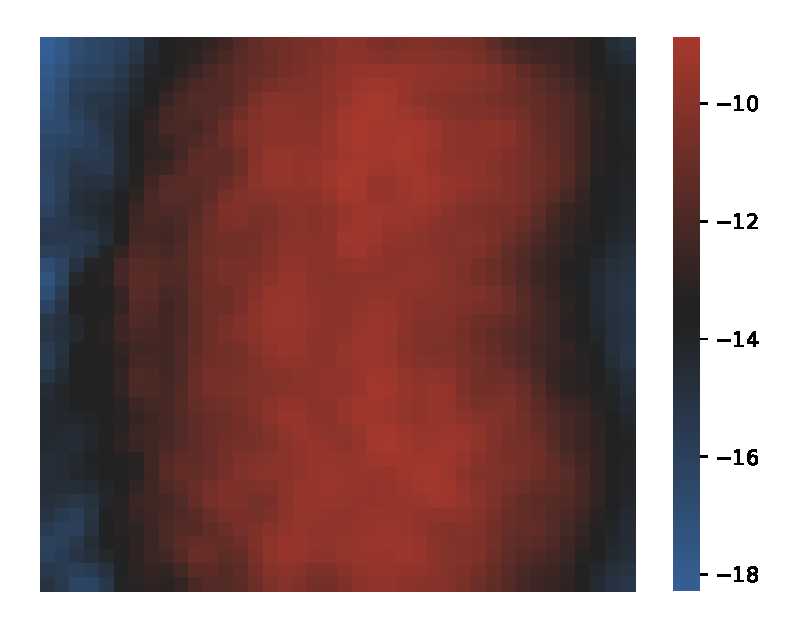
\includegraphics[width=.3\linewidth]{figures/spp/car_sdf_slices/x_0.eps}&
		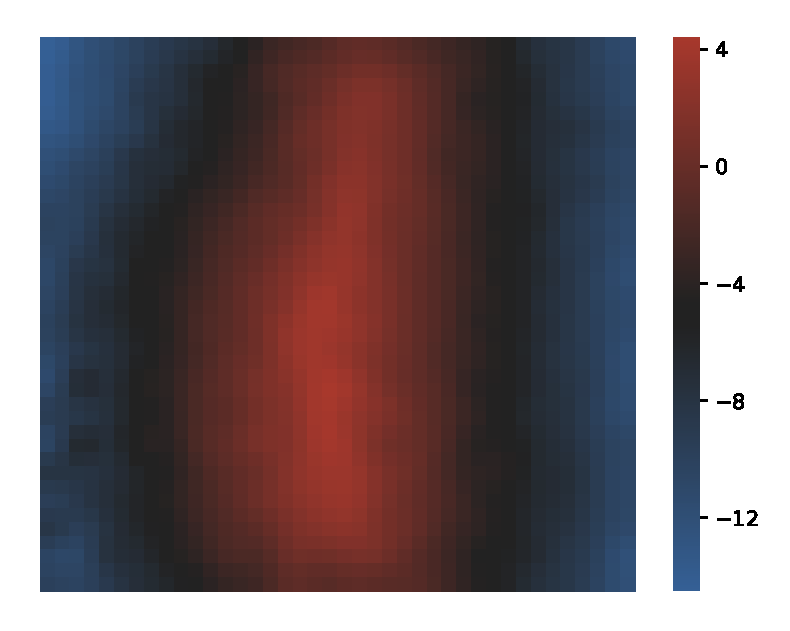
\includegraphics[width=.3\linewidth]{figures/spp/car_sdf_slices/x_10.eps}&
		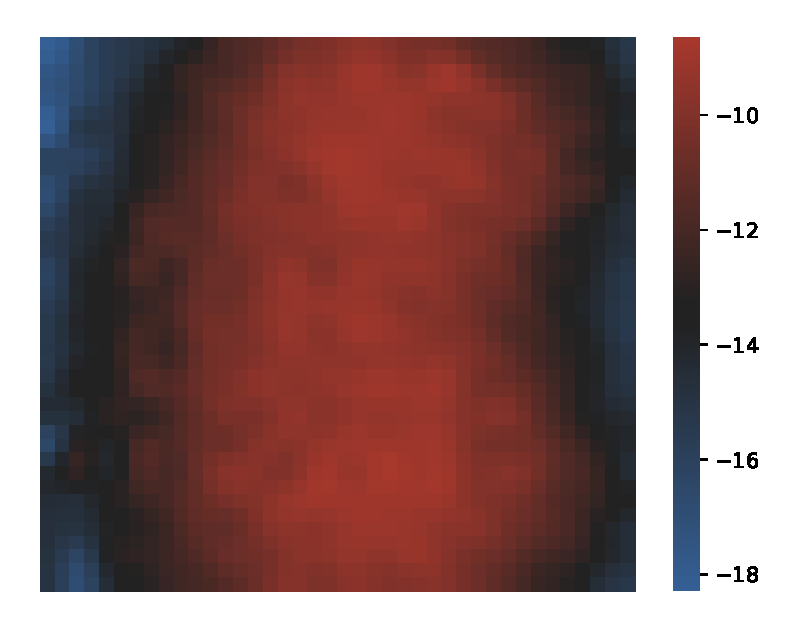
\includegraphics[width=.3\linewidth]{figures/spp/car_sdf_slices/x_19.eps}\\
    (a) & (b) & (c) \\
    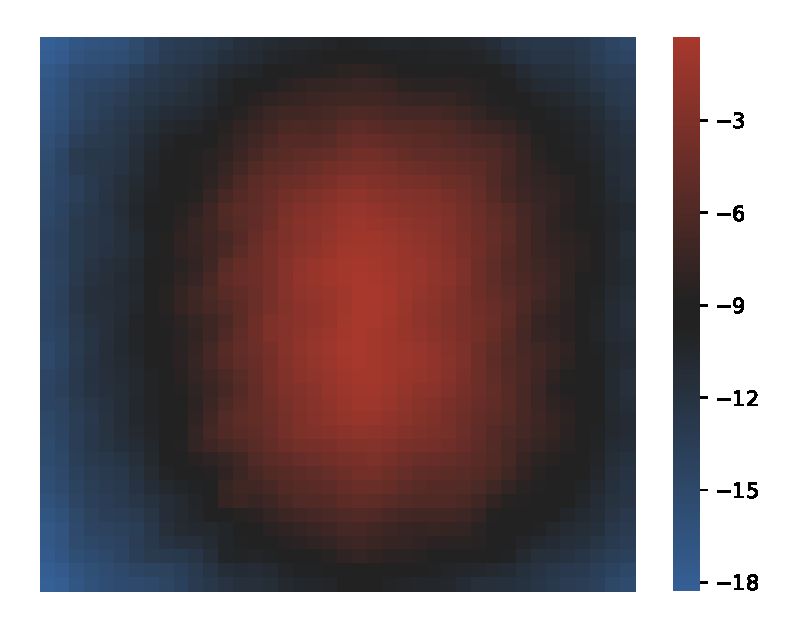
\includegraphics[width=.3\linewidth]{figures/spp/car_sdf_slices/y_0.eps}&
		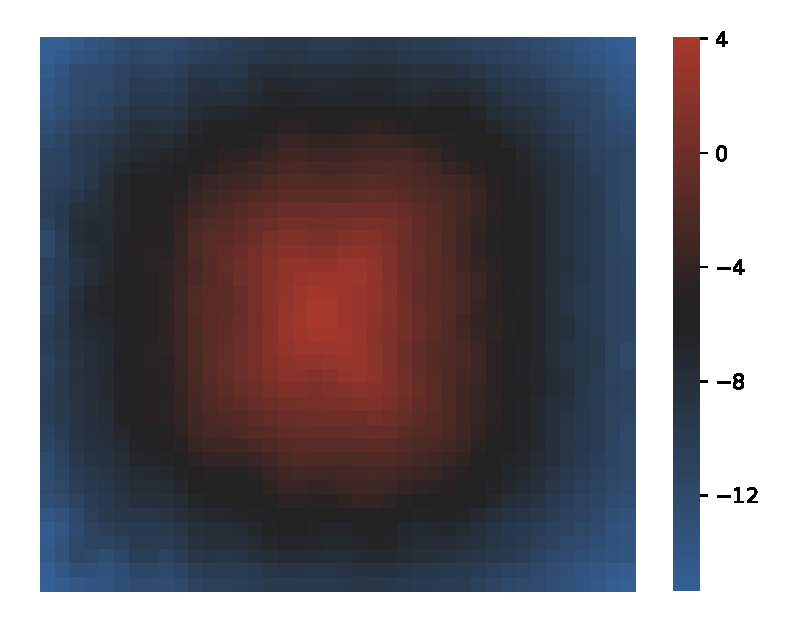
\includegraphics[width=.3\linewidth]{figures/spp/car_sdf_slices/y_10.eps}&
		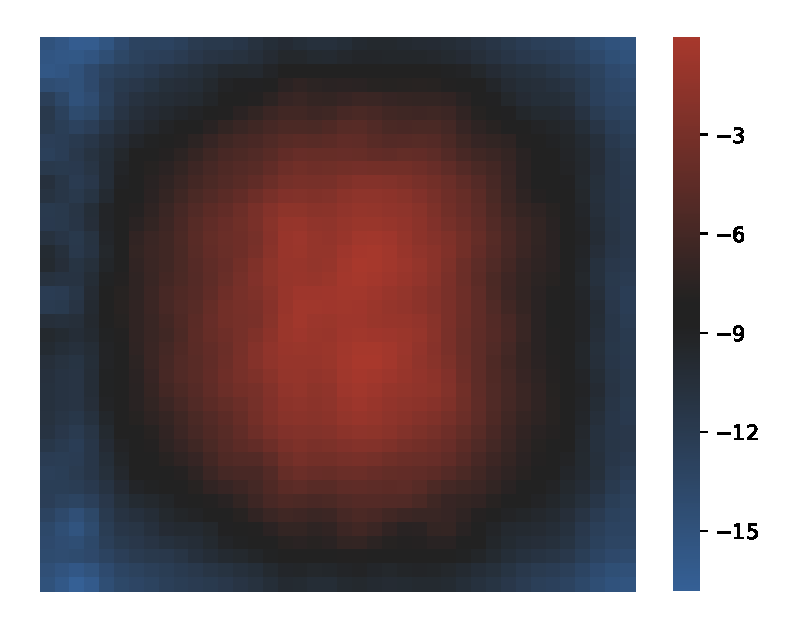
\includegraphics[width=.3\linewidth]{figures/spp/car_sdf_slices/y_19.eps}\\
    (d) & (e) & (f) \\
    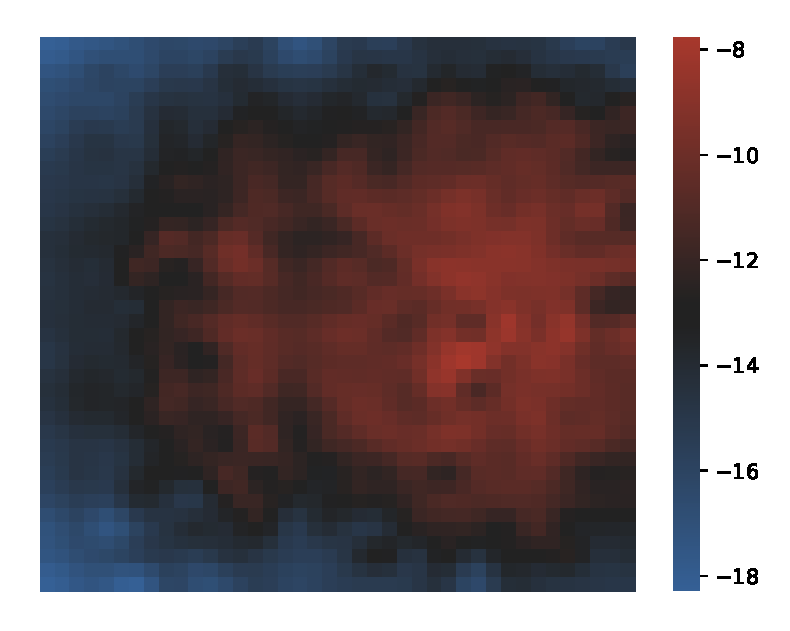
\includegraphics[width=.3\linewidth]{figures/spp/car_sdf_slices/z_0.eps}&
		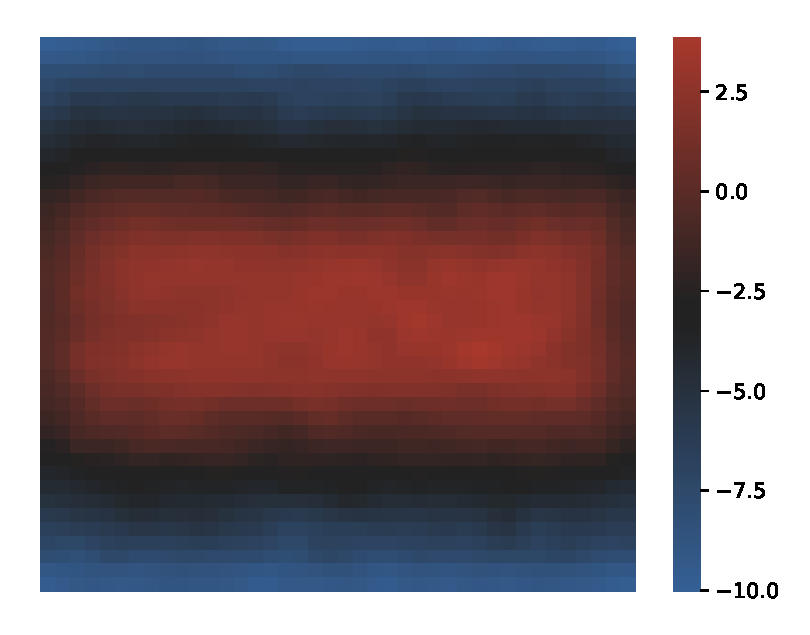
\includegraphics[width=.3\linewidth]{figures/spp/car_sdf_slices/z_10.eps}&
		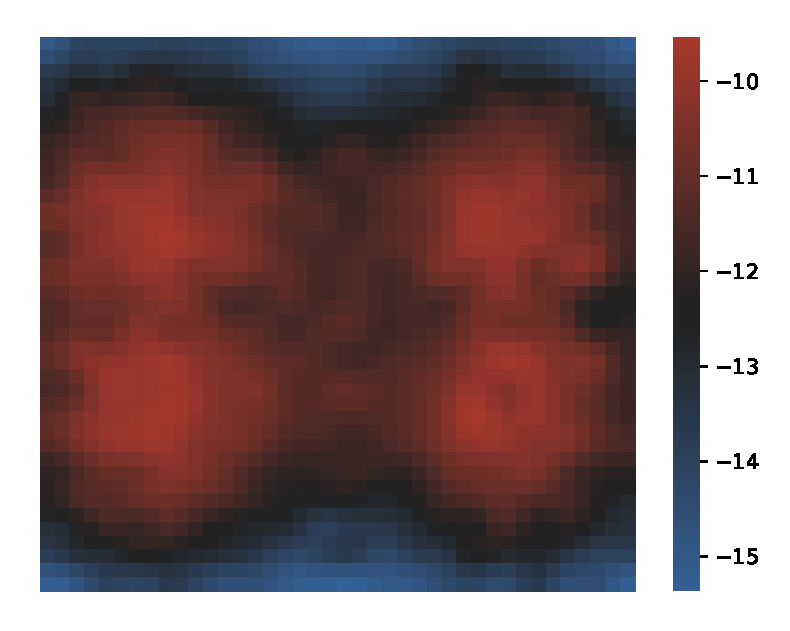
\includegraphics[width=.3\linewidth]{figures/spp/car_sdf_slices/z_19.eps}\\
    (g) & (h) & (i)
  \end{tabular}
  \caption[SDF Slices Generated by DCT]
  {
    \begin{tabular}[t]{@{}l@{}}
      Slices of a Signed Distance Function embedding \( \bm{\Phi} \in \mathbb{R}^{20 \times 20 \times 20} \)
      of a\\ car at slices 0, 10 and 19:\\
      (a, b, c) Along the \(x\) axis.\\
      (d, e, f) Along the \(y\) axis.\\
      (g, h, i) Along the \(z\) axis.
    \end{tabular}
  }
~\label{figure:spp_sdf_slices}
\end{figure}

The voxels of an input SDF \( \bm{V} \) under the DCT (for model training) are thus given 
as follows in Equation~\ref{eqn:spp_dct}.
\begin{align}
  \label{eqn:spp_dct}
  % Line 1.
  \bm{\Psi}_{x, y, z} ={}& \bm{V}_{x, y, z} \Bigg[
  \sum_{x=0}^{N-1} \cos \Big[ \frac{\pi}{N} \big[ x + \frac{1}{2} \big] x \Big]
  \sum_{y=0}^{N-1} \cos \Big[ \frac{\pi}{N} \big[ y + \frac{1}{2} \big] y \Big]
  \sum_{z=0}^{N-1} \cos \Big[ \frac{\pi}{N} \big[ z + \frac{1}{2} \big] z \Big] \Bigg]\\
  % Line 2.
  ={}& \bm{V}_{x, y, z} \Bigg[
  \sum_{x=0}^{N-1} \cos \Big[ \frac{\pi \big( x^{2} + \frac{x}{2} \big)}{N} \Big]
  \sum_{y=0}^{N-1} \cos \Big[ \frac{\pi \big( y^{2} + \frac{y}{2} \big)}{N} \Big]
  \sum_{z=0}^{N-1} \cos \Big[ \frac{\pi \big( z^{2} + \frac{z}{2} \big)}{N} \Big] \Bigg]\\
  % Line 3.
  ={}& \sum_{x=0}^{N-1} \sum_{y=0}^{N-1} \sum_{z=0}^{N-1} \bm{V}_{x, y, z}
  \cos \Big[ \frac{\pi \big( x^{2} + \frac{x}{2} \big)}{N} \Big]
  \cos \Big[ \frac{\pi \big( y^{2} + \frac{y}{2} \big)}{N} \Big]
  \cos \Big[ \frac{\pi \big( z^{2} + \frac{z}{2} \big)}{N} \Big]
\end{align}

It follows that for a predicted posterior mean \( \bm{f}^{\star} \), as outlined in 
Equation~\ref{eqn:spp_gp_posterior_draw}, the voxels of the SDF corresponding to the 
estimation \( \bm{f}^{\star} \) may be extracted via the IDCT as follows in 
Equation~\ref{eqn:spp_idct}.
\begin{equation}
  \label{eqn:spp_idct}
  \bm{\Phi}_{x, y, z} = \sum_{x=0}^{N-1} \sum_{y=0}^{N-1} \sum_{z=0}^{N-1} 
  \bm{f}^{\star}_{x, y, z}
  \cos \Big[ \frac{\pi \big( x^{2} + \frac{x}{2} \big)}{N} \Big]
  \cos \Big[ \frac{\pi \big( y^{2} + \frac{y}{2} \big)}{N} \Big]
  \cos \Big[ \frac{\pi \big( z^{2} + \frac{z}{2} \big)}{N} \Big]
\end{equation}

An example of how the geometric detail of the decompressed model varies with the number 
of harmonics used, \( N \), is given in Figure~\ref{figure:spp_sdf_diff_harmonics}.
\begin{figure}[!htbp]
  \centering
  \begin{tabular}{ccc}
    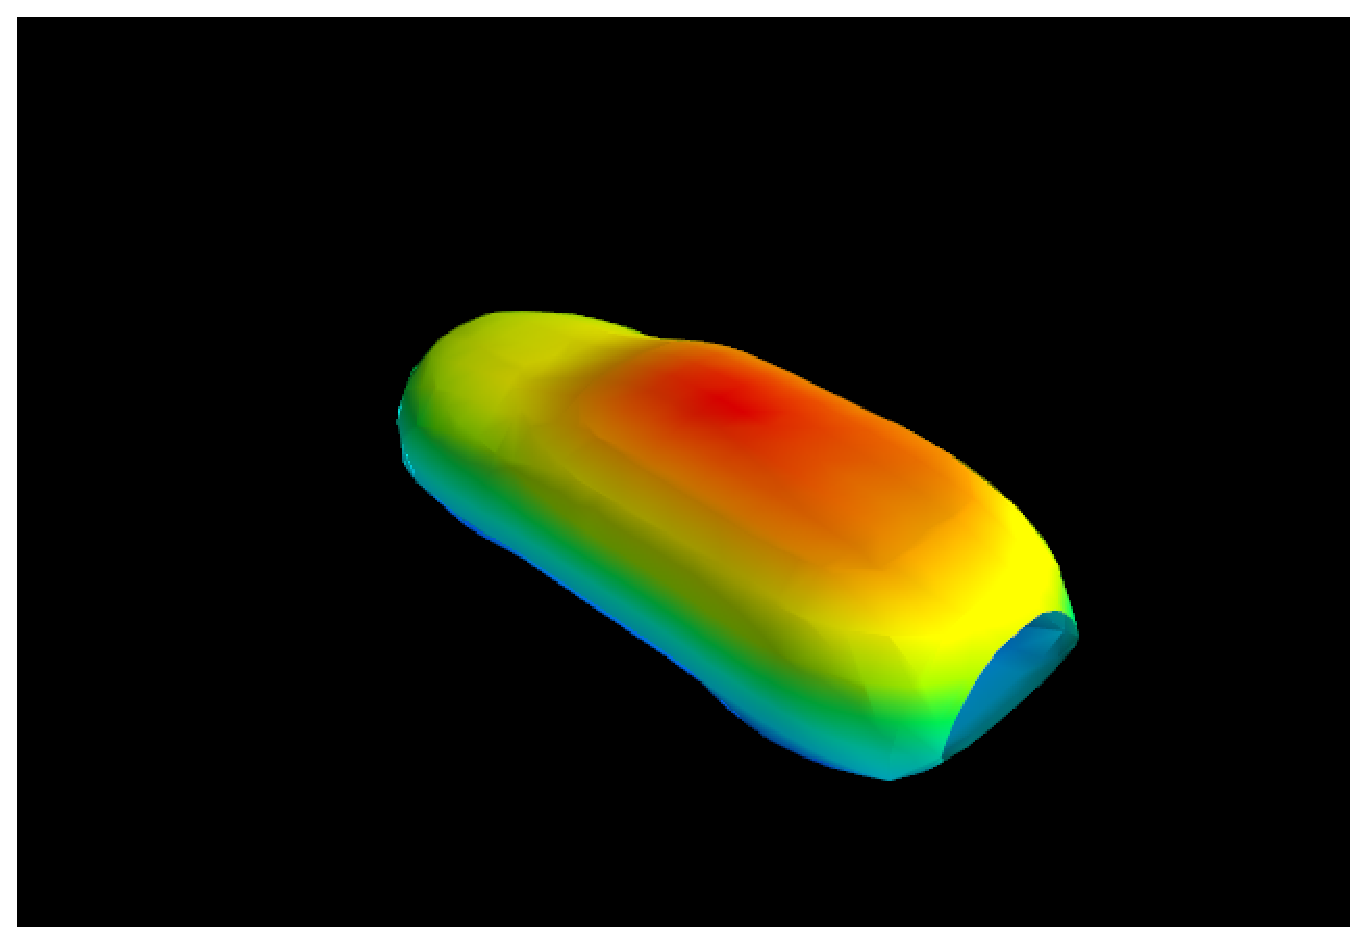
\includegraphics[width=.4\linewidth]{figures/spp/differing_harmonics/1.eps}&
		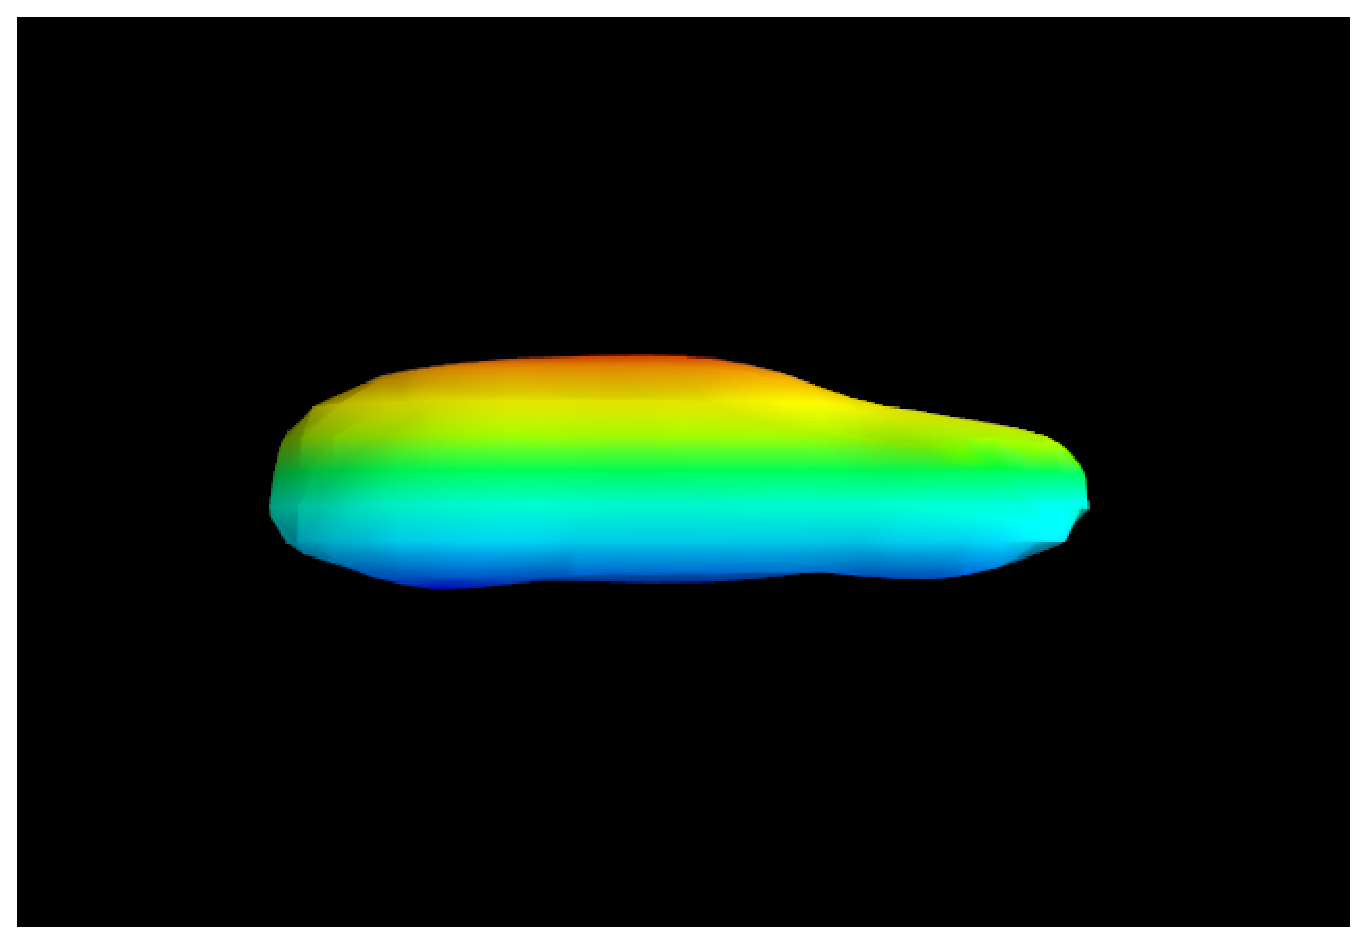
\includegraphics[width=.4\linewidth]{figures/spp/differing_harmonics/1_side.eps}\\
    (a) & (b) \\
    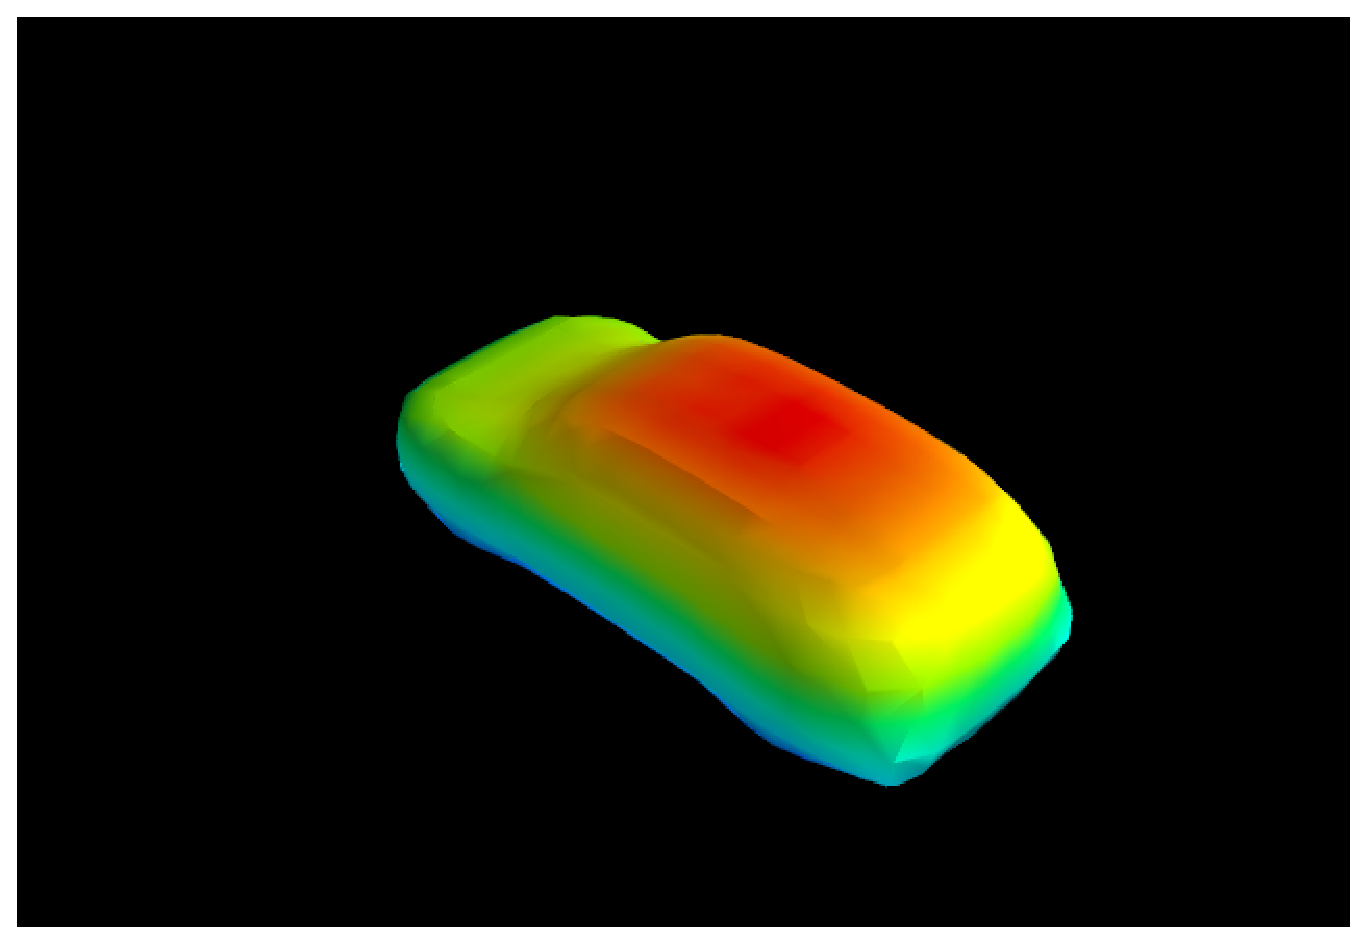
\includegraphics[width=.4\linewidth]{figures/spp/differing_harmonics/3.eps}&
		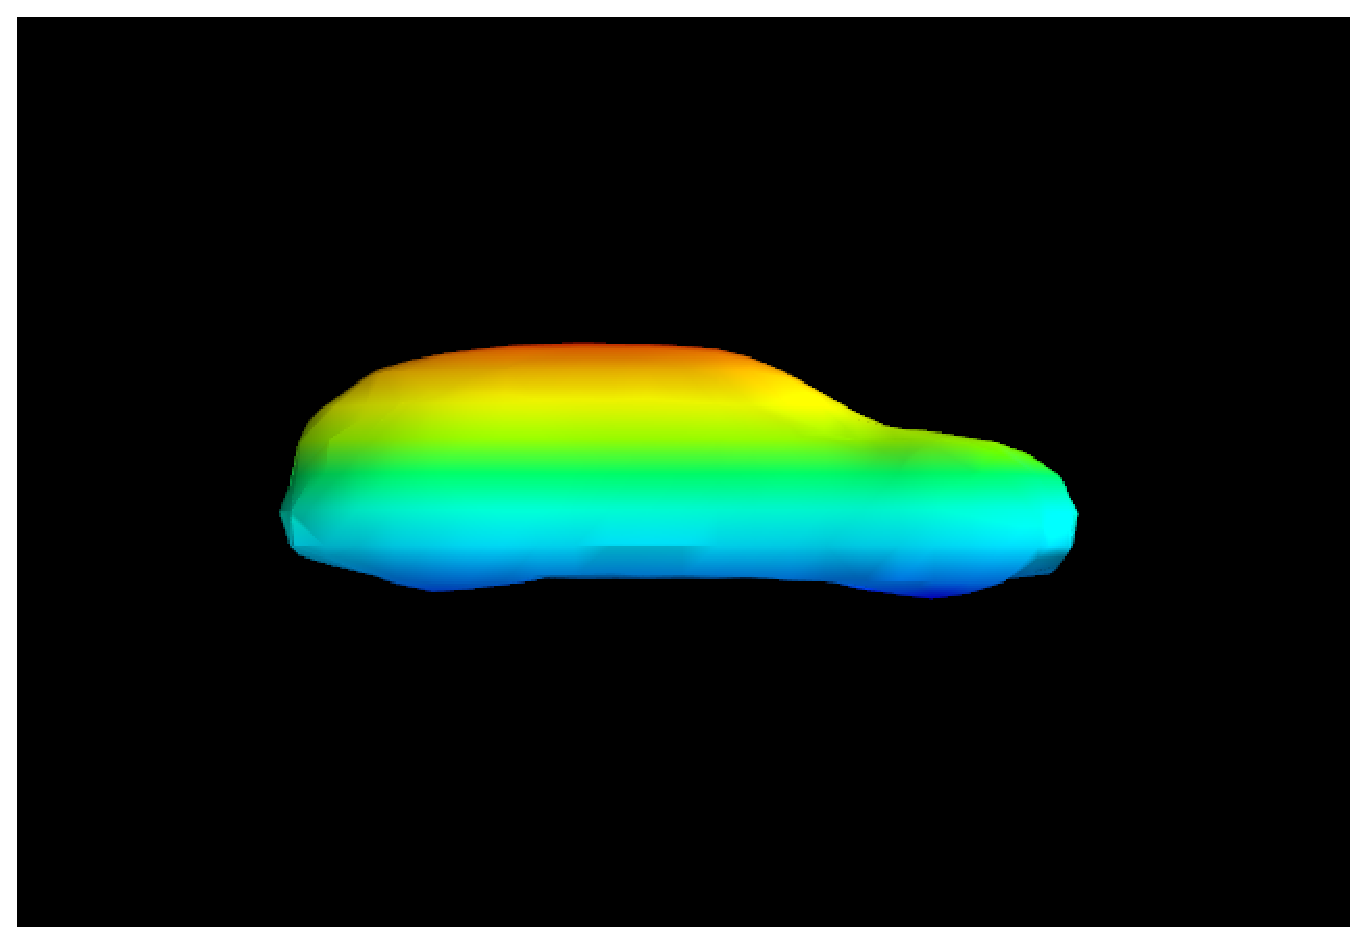
\includegraphics[width=.4\linewidth]{figures/spp/differing_harmonics/3_side.eps}\\
    (c) & (d) \\
    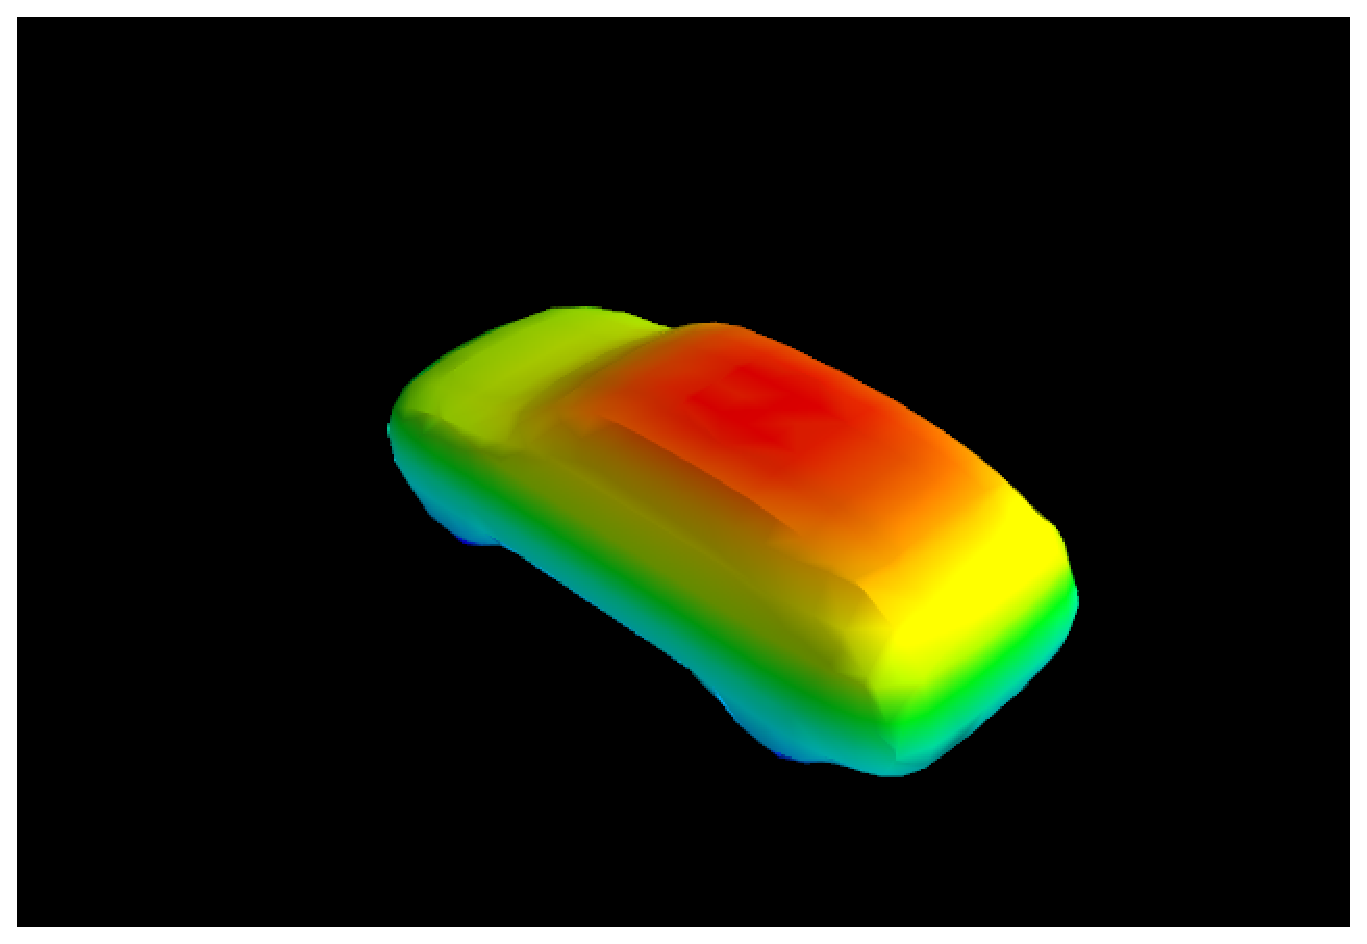
\includegraphics[width=.4\linewidth]{figures/spp/differing_harmonics/all.eps}&
		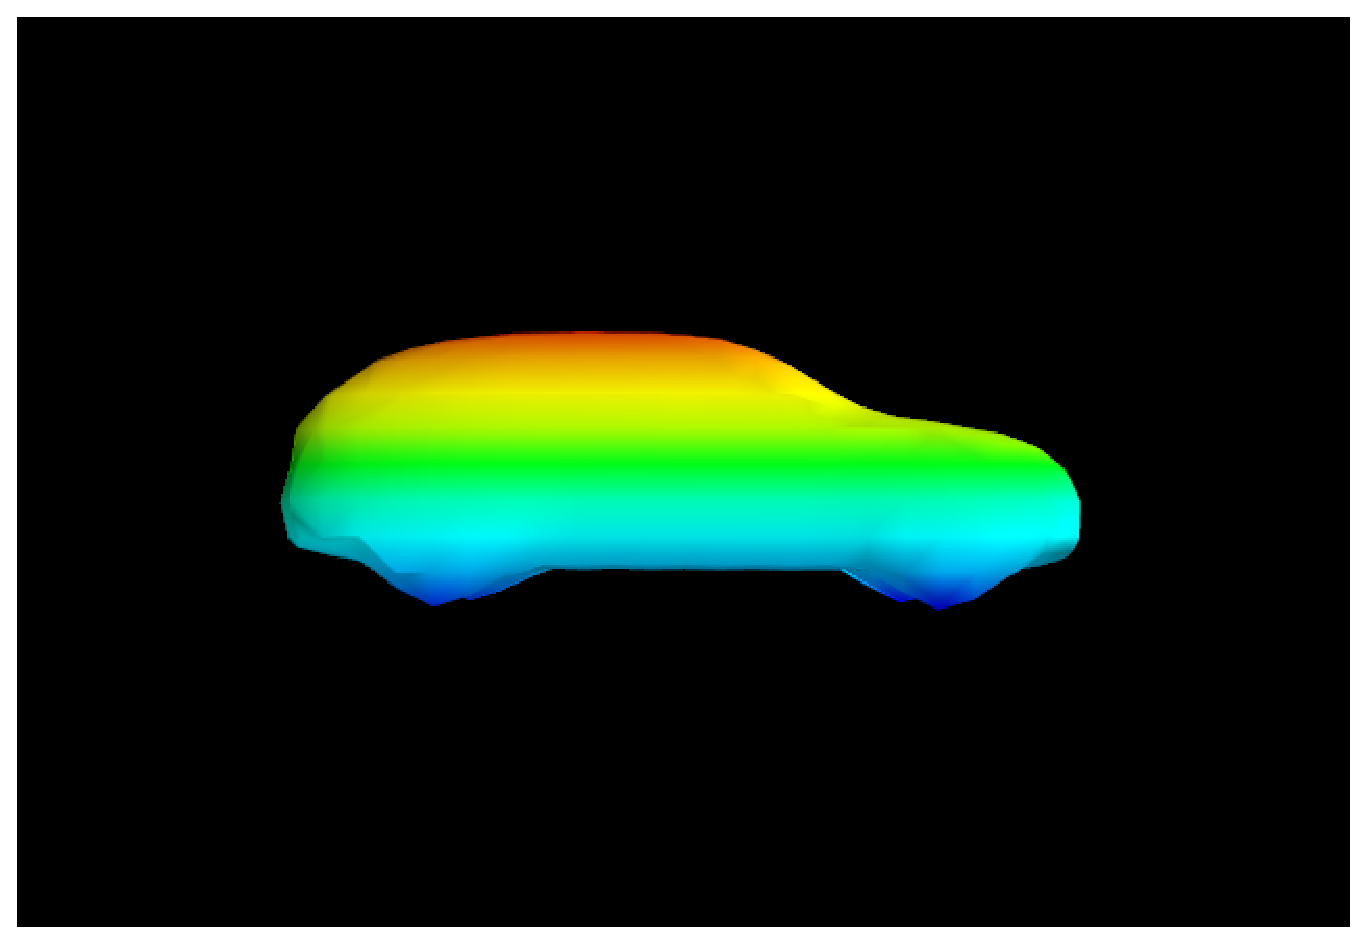
\includegraphics[width=.4\linewidth]{figures/spp/differing_harmonics/all_side.eps}\\
    (e) & (f)
  \end{tabular}
  \caption[SDF's generated with differing DCT harmonics.]
  {
    \begin{tabular}[t]{@{}l@{}}
      The effect of varying the number of DCT harmonics on the resultant 3D shape is shown for:\\
      (a, b) One DCT harmonic.\\
      (c, d) Three DCT harmonics.\\
      (e, f) All DCT harmonics.\\
    \end{tabular}
  }
~\label{figure:spp_sdf_diff_harmonics}
\end{figure}

\subsection{Signed Distance Function Gradient}
~\label{subsec:spp_sdf_grad}
The SDF \( \bm{\Phi} \) generated by the IDCT given in Equation~\ref{eqn:spp_idct} must be 
differentiable with respect to the posterior mean \( \bm{f}^{\star} \) for backpropagation 
training of the model. The gradient of the SDF \( \bm{\Phi} \) outlined in 
Equation~\ref{eqn:spp_idct} is derived as follows in Equation~\ref{eqn:spp_idct_grad}. 
For notational clarity, the DCT coefficients are defined as follows in Equation
~\ref{eqn:spp_dct_coeff}
\begin{equation}
  \label{eqn:spp_dct_coeff}
  \zeta(x, y, z) = 
  \cos \Big[ \frac{\pi \big( x^{2} + \frac{x}{2} \big)}{N} \Big]
  \cos \Big[ \frac{\pi \big( y^{2} + \frac{y}{2} \big)}{N} \Big]
  \cos \Big[ \frac{\pi \big( z^{2} + \frac{z}{2} \big)}{N} \Big]
\end{equation}
\begin{align}
  \label{eqn:spp_idct_grad}
  % Line 1.
  \frac{\partial \bm{\Phi}}{\partial \bm{f}_{x, y, z}^{\star}} ={}&
  \frac{\partial}{\partial \bm{f}_{x, y, z}^{\star}}
  \sum_{x=0}^{N-1} \sum_{y=0}^{N-1} \sum_{z=0}^{N-1} 
  \bm{f}^{\star}_{x, y, z} \zeta(x, y, z)\\
  % Line 2.
  ={}& \sum_{x=0}^{N-1} \sum_{y=0}^{N-1} \sum_{z=0}^{N-1} 
  \frac{\partial}{\partial \bm{f}_{x, y, z}^{\star}} \bm{f}^{\star}_{x, y, z}
  \zeta(x, y, z)\\
  % Line 3.
  ={}& \sum_{x=0}^{N-1} \sum_{y=0}^{N-1} \sum_{z=0}^{N-1} \Bigg[
    \Bigg[ 
      \frac{\partial}{\partial \bm{f}_{x, y, z}^{\star}} \bm{f}^{\star}_{x, y, z} 
    \Bigg] \zeta(x, y, z)
    + \bm{f}_{x, y, z}^{\star} \frac{\partial \zeta}{\partial \bm{f}_{x, y, z}^{\star}}
  \Bigg]\\
  % Line 4.
  ={}& \sum_{x=0}^{N-1} \sum_{y=0}^{N-1} \sum_{z=0}^{N-1}
  \nabla \bm{f}_{x, y, z}^{\star} \zeta(x, y, z)\\
  % Line 5.
  ={}& \sum_{x=0}^{N-1} \sum_{y=0}^{N-1} \sum_{z=0}^{N-1} 
  \nabla \bm{f}^{\star}_{x, y, z}
  \cos \Big[ \frac{\pi \big( x^{2} + \frac{x}{2} \big)}{N} \Big]
  \cos \Big[ \frac{\pi \big( y^{2} + \frac{y}{2} \big)}{N} \Big]
  \cos \Big[ \frac{\pi \big( z^{2} + \frac{z}{2} \big)}{N} \Big]
\end{align}
From Equation~\ref{eqn:spp_idct_grad} it is evident that the partial derivative 
\( \frac{\partial \bm{\Phi}}{\partial \bm{f}_{x, y, z}^{\star}} \) is trivial 
to compute as the derivative of the IDCT is simply the IDCT of the derivative. 
Furthermore, the gradient of the posterior mean is trivial to compute, as shown 
in Equation~\ref{eqn:spp_pos_mean_grad}.

\section{Pose Estimation}
~\label{sec:spp_pose_estim}
The parameters of the \( \mathbb{SE}(3) \) pose applied to the predicted shape are obtained 
from a fully connected component of the model outlined in Figure~\ref{figure:spp_pipeline}, as with the 
latent pose point of Section~\ref{subsec:sdf_extraction}. The form of the \( \mathbb{SE}(3) \) pose is 
analogous to the Rodrigues parameterisation outlined in Section~\ref{subsub:moseg_static_camera_poserec}.

The three rotational parameters \( \alpha \), \( \beta \) and \( \gamma \) are predicted by 
the pose network component of the model on the interval \( [0, 2\pi) \). The translation parameters 
however do not have their output restricted. It should be noted that the pose Jacobians are of the 
same form as those outlined in Equations~\ref{eqn:rot_jac} and~\ref{eqn:trans_jac}.

\section{Rendering}
~\label{sec:spp_rendering}
The dynamic SLAM and object reconstruction works of Chapters~\ref{chap:moseg} and~\ref{chap:probobj}, 
both rely on Raycasting to obtain a rendering of a surface embedded within an implicit volume, under 
some estimated pose. The approach taken in this chapter is very similar. 

Raycasting is first and foremost used in the model outlined in Section~\ref{sec:spp_algorithm} for 
visualisation purposes, to render the estimated shape under the estimated pose for an instantaneous scene 
view. In Chapters~\ref{chap:moseg} and~\ref{chap:probobj}, the output rendering is also used for frame-wise 
evaluation and optimisation of the pose energy function. However, as the approach outlined in this chapter 
does not assume temporal consistency, the requirements for optimisation differ.

As the model outlined in Section~\ref{sec:spp_algorithm} relies on the backpropagation of gradients for it's 
training, the rendering module must be differentiable for the backward pass. As such, this section outlines a 
simple formulation of differentiable Raycasting, inspired by the work of \textit{Prisacariu et al}
~\cite{Prisacariu2011}. In addition to generating a shaded rendering, the proposed approach generates a 
probabilistic map. For a review of the general Raycasting algorithm, refer to 
Section~\ref{subsec:moseg_static_rendering}.

By accumulating log probabilities of voxels visited on traversal of the ray, a differentiable representation 
of the process can be obtained. However, this relies on the use of a differentiable PMF\@. As with the approach 
to object reconstruction outlined in Chapter~\ref{chap:probobj}, the desired behaviour is that the distribution 
shall encode the probability of a voxel being very close to the isosurface. As such, the Log-Sigmoid of Equation
~\ref{eqn:probobj_surface_prior_cdf} is used. Thus, for a pixel location \( [x, y] \), the output probabistic 
value is as follows in Equation~\ref{eqn:spp_diff_raycast}.
\begin{equation}
~\label{eqn:spp_diff_raycast}
\mathcal{R}(x, y) = \sum_{v \in \mathcal{V}} \ln P(v)
\end{equation}

In Equation~\ref{eqn:spp_diff_raycast}, \( \mathcal{V} \) is the set of voxels in the SDF \( \bm{\Phi} \) that 
intersect the ray from the given pixel in the image frame. The gradient of the \( \ln P(v) \) term in 
Equation~\ref{eqn:spp_diff_raycast} if the form given in Equation~\ref{eqn:probobj_log_post_rot_grad}.

\section{Information Theoretic Loss}
~\label{sec:spp_loss}
As outlined in Section~\ref{sec:spp_algorithm}, the proposed model is trained in a semi-supervised 
manner on an information theoretic loss. For each of the left and right networks, the loss is 
quantified by the Kullback-Leibler (KL) Divergence between the appearances of the initial detection region 
and the prediction region (the image space in which the predicted shape is rendered to). Appearances for 
each of the regions are quantified by simple image statistics. The intuition behind such a loss is that 
for an optimal predicted shape and pose, the KL Divergences will be minimal due to the very high overlap 
between detection and prediction.

Additionally, to reduce divergence during training between the left and right models of the Siamese 
architecture, the Jensen-Shannon Divergence (JSD) is applied to the predictions of the left and right outputs.
The overall loss is thus given in Equation~\ref{eqn:spp_overall_loss}.
\begin{align}
  \label{eqn:spp_overall_loss}
  % Line 1.
  \mathcal{L}(.) &{}= \frac{1}{2} \Bigg[
    \mathbb{KL}(\bm{P} \vert \bm{Q}) + \mathbb{KL}(\bar{\bm{P}} \vert \bar{\bm{Q}})
  \Bigg]
  + \mathbb{JSD}(\bm{Q}, \bar{\bm{Q}})\\
  % Line 2.
  &{}= 
  \begin{aligned}[t]
    {}& \frac{1}{2} \Bigg[
      -\sum_{d = 0}^{D} \ln{(\bm{Q}_{d})}\bm{P}_{d} + \sum_{d = 0}^{D} \bm{P}_{d}\ln{\bm{P}_{d}}
      -\sum_{d = 0}^{D} \ln{(\bar{\bm{Q}}_{d})}\bar{\bm{P}}_{d} + \sum_{d = 0}^{D} \bar{\bm{P}}_{d}\ln{\bar{\bm{P}}_{d}}
    \Bigg]\\
    {}& + \frac{1}{2} \Bigg[
      -\sum_{d = 0}^{D} \ln{(\bm{Q}_{d})}\bm{M}_{d} + \sum_{d = 0}^{D} \bm{M}_{d}\ln{\bm{M}_{d}}
      -\sum_{d = 0}^{D} \ln{(\bar{\bm{Q}}_{d})}\bm{M}_{d} + \sum_{d = 0}^{D} \bm{M}_{d}\ln{\bm{M}_{d}}
    \Bigg]
  \end{aligned}\\
  \shortintertext{Where \( \bm{M} = \frac{1}{2} (\bm{Q} + \bar{\bm{Q}}) \)}\\
  % Line 3.
  {}&= \frac{1}{2} \sum_{d = 0}^{D}
    \begin{aligned}[t]
    \Bigg[ {}&
    -\ln{(\bm{Q}_{d})}\bm{P}_{d} + \bm{P}_{d}\ln{\bm{P}_{d}}
    -\ln{(\bar{\bm{Q}_{d}})}\bar{\bm{P}_{d}} + \bar{\bm{P}}_{d}\ln{\bar{\bm{P}}_{d}}\\
    {}& -\ln{(\bm{Q}_{d})}\bm{M}_{d} -\ln{(\bar{\bm{Q}_{d}})}\bm{M}_{d} + 2\bm{M}_{d}\ln{\bm{M}_{d}}
    \Bigg]
    \end{aligned}
\end{align}

The loss function given in Equation~\ref{eqn:spp_overall_loss} makes use of the mode seeking~\cite{Minka2005} 
\textit{forward} KL Divergence from the observed detection regions to the rendered (predicted) 
regions. The motivation behind which is to quantify, for each of the left and right networks, how 
much information is lost for the currently predicted shapes and \( \mathbb{SE}(3) \) poses. To 
enforce consistency between the left and right networks, the JSD is used, as unlike the KL Divergence, 
it is \textit{symmetric} and \( \bm{Q} \) need not approximate \( \bar{Q} \), any better than 
\( \bar{\bm{Q}} \) need approximate \( \bm{Q} \).

\subsection{Information Theoretic Loss Gradient}
~\label{subsec:spp_inf_loss_grad}
As with the model components outlined in Sections~\ref{sec:spp_latent_shape_est},~\ref{sec:spp_pose_estim} 
and~\ref{sec:spp_rendering}, the loss of the model also requires differentiability for backpropagation. As such, 
the gradient \( \frac{\partial \mathcal{L}}{\partial \bm{Q}} \) is as follows in Equation~\ref{eqn:spp_loss_grad}.
\begin{align}
  \label{eqn:spp_loss_grad}
  % Line 1.
  \frac{\partial \mathcal{L}}{\partial \bm{Q}} {}&=
  \frac{1}{2} \sum_{d = 0}^{D} \frac{\partial}{\partial \bm{Q}}
  \begin{aligned}[t]
    \Bigg[ {}&
      -\ln{(\bm{Q}_{d})}\bm{P}_{d} + \bm{P}_{d}\ln{\bm{P}_{d}}
      -\ln{(\bar{\bm{Q}_{d}})}\bar{\bm{P}_{d}} + \bar{\bm{P}}_{d}\ln{\bar{\bm{P}}_{d}}
      -\ln{(\bm{Q}_{d})}\bm{M}_{d}\\
      {}& 
      -\ln{(\bar{\bm{Q}_{d}})}\bm{M}_{d} + 2\bm{M}_{d}\ln{\bm{M}_{d}}
    \Bigg]
  \end{aligned}\\
  % Line 2.
  {}&= \frac{1}{2} \sum_{d = 0}^{D}
  \begin{aligned}[t]
    \Bigg[ {}&
      -\frac{\partial}{\partial \bm{Q}_{d}} \ln{(\bm{Q}_{d})}\bm{P}_{d} 
      +\frac{\partial}{\partial \bm{Q}_{d}} \bm{P}_{d}\ln{\bm{P}_{d}}
      -\frac{\partial}{\partial \bm{Q}_{d}} \ln{(\bar{\bm{Q}_{d}})}\bar{\bm{P}_{d}}
      +\frac{\partial}{\partial \bm{Q}_{d}} \bar{\bm{P}}_{d}\ln{\bar{\bm{P}}_{d}}\\
      {}&
      -\frac{\partial}{\partial \bm{Q}_{d}} \ln{(\bm{Q}_{d})}\bm{M}_{d} 
      -\frac{\partial}{\partial \bm{Q}_{d}} \ln{(\bar{\bm{Q}_{d}})}\bm{M}_{d}
      +2 \frac{\partial}{\partial \bm{Q}_{d}} \bm{M}_{d}\ln{\bm{M}_{d}}
    \Bigg]
  \end{aligned}\\
  % Line 3.
  {}&= \frac{1}{2} \sum_{d = 0}^{D}
  \begin{aligned}[t]
    \Bigg[ {}&
      -\frac{\bm{P}_{d}}{\bm{Q}_{d}}
      -\bm{M}_{d} \frac{\partial}{\partial \bm{Q}_{d}} \ln{\bm{Q}_{d}}
      -\ln{\bm{Q}_{d}} \frac{\partial \bm{M}_{d}}{\partial \bm{Q}_{d}}
      -\ln{\bar{\bm{Q}}} \frac{\partial \bm{M}_{d}}{\partial \bm{Q}_{d}}
      +2 \frac{\partial \bm{M}_{d}}{\partial \bm{Q}_{d}} \ln{\bm{M}_{d}}\\
      {}&
      +2 \bm{M}_{d} \frac{\partial}{\partial \bm{Q}_{d}} \ln{\bm{M}_{d}}
    \Bigg]
  \end{aligned}\\
\shortintertext{Where \( \bm{M} = \frac{1}{2} (\bm{Q} + \bar{\bm{Q}}) \)}\\
  % Line 4.
  {}&= \frac{1}{2} \sum_{d = 0}^{D}
  \begin{aligned}[t]
    \Bigg[ {}&
      -\frac{\bm{P}_{d}}{\bm{Q}_{d}}
      -\frac{\bm{M}_{d}}{\bm{Q}_{d}}
      +\ln{\bm{Q}_{d}} \frac{\partial \bm{M}_{d}}{\partial \bm{Q}_{d}}
      -\ln{\bar{\bm{Q}_{d}}} \frac{\partial \bm{M}_{d}}{\partial \bm{Q}_{d}}
      +2 \frac{\partial \bm{M}_{d}}{\partial \bm{Q}_{d}} \ln{\bm{Q}_{d}}\\
      {}&
      +2 \bm{M}_{d} \frac{\partial}{\partial \bm{Q}_{d}} \ln{\bm{M}_{d}}
    \Bigg]
  \end{aligned}\\
  % Line 5.
  {}&= \frac{1}{2} \sum_{d = 0}^{D}
  \begin{aligned}[t]
    \Bigg[ {}&
      -\frac{\bm{P}_{d} + \bm{M}_{d}}{\bm{Q}_{d}}
      +\frac{\ln{\bm{Q}_{d} - \ln{\bar{\bm{Q}}_{d}}}}{2}
      +\ln{\bm{M}_{d}} 
      +\frac{2\bm{M}_{d}}{\bm{Q}_{d} + \bar{\bm{Q}}_{d}}
    \Bigg]
  \end{aligned}\\
  % Line 6.
  {}&= \frac{1}{2} \sum_{d = 0}^{D}
  \begin{aligned}[t]
    \Bigg[ {}&
      -\frac{\bm{P}_{d} + \frac{\bm{Q}_{d} + \bar{\bm{Q}}_{d}}{2}}{\bm{Q}_{d}}
      +\frac{\ln{\bm{Q}_{d}} + \ln{\bar{\bm{Q}}_{d}}}{2}
      +\ln{\frac{\bm{Q}_{d} + \bar{\bm{Q}}_{d}}{2}}
    \Bigg]
  \end{aligned}\\
  % Line 7.
  {}&= \frac{1}{2} \sum_{d = 0}^{D}
  \begin{aligned}[t]
    \Bigg [
      -\frac{1}{2 \bm{Q}_{d}} \Bigg[
        2 \bm{P}_{d} + \bm{Q}_{d} \big( 1 + \ln{\bar{\bm{Q}}_{d}} \big)
        + \bm{Q}_{d} \ln{\bm{Q}_{d}}
        + \bar{\bm{Q}}_{d}
      \Bigg]
      +\ln{\frac{\bm{Q}_{d} + \bar{\bm{Q}}_{d}}{2}}
    \Bigg]
  \end{aligned}
\end{align}

\section{Gradients for Training With Backpropagation}
~\label{sec:spp_backprop}
With the gradients of the model components now derived, the gradient update to the neural network component 
of the model may be given. As the proposed model is optimised using the Backpropagation algorithm, 
the gradient update for layer \( n - m \) is computed by applying the chain rule to layer \( n \), 
successively working backwards to layer \( n - m \). As such, the gradient for the non CNN components 
with respect to the CNN output for pose \( \mathcal{O}_{p} \), is given as follows in Equation
~\ref{eqn:spp_grad_chain_pose}.
\begin{equation}
  \label{eqn:spp_grad_chain_pose}
  \frac{\partial \mathcal{L}}{\partial \mathcal{O}_{p}} = 
  \frac{1}{2} \sum_{\omega \in \{L, R\}} \Bigg[
    \frac{\partial \mathcal{L}}{\partial \mathcal{R}_{\omega}}
    \frac{\partial \mathcal{R}_{\omega}}{\partial \bm{T}_{\omega}}
    \frac{\partial \bm{T}_{\omega}}{\partial \mathcal{O}_{p}}
  \Bigg]
\end{equation}

In Equation~\ref{eqn:spp_grad_chain_pose}, \( \mathcal{L} \) is the information theoretic loss 
given in Equation~\ref{eqn:spp_overall_loss} of Section~\ref{sec:spp_loss}.
\( \mathcal{R} \) is the rendering of the predicted shape \( \bm{\Phi} \) under the predicted 
pose \( \bm{T} \) outlined in Section~\ref{sec:spp_rendering}. \( \bm{T} \) is the 
\( \mathbb{SE}(3) \) pose outlined in Section~\ref{sec:spp_pose_estim}. The gradient with respect 
to the latent shape point generated by CNN output \( \mathcal{O}_{l} \) may also be found in the same 
manner and is given in Equation~\ref{eqn:spp_grad_chain_latent}.
\begin{equation}
  \label{eqn:spp_grad_chain_latent}
  \frac{\partial \mathcal{L}}{\partial \mathcal{O}_{l}} = 
  \frac{1}{2} \sum_{\omega \in \{L, R\}} \Bigg[
    \frac{\partial \mathcal{L}}{\partial \mathcal{R}_{\omega}}
    \frac{\partial \mathcal{R}_{\omega}}{\partial \mathcal{\bm{\Phi}}_{\omega}}
    \frac{\partial \bm{\Phi}_{\omega}}{\partial \bm{f}^{\star}_{\omega}}
    \frac{\partial \bm{f}^{\star}_{\omega}}{\partial \mathcal{O}_{l}}
  \Bigg]
\end{equation}

In Equation~\ref{eqn:spp_grad_chain_latent}, \( \mathcal{L} \) and \( \mathcal{R} \) 
are as in Equation~\ref{eqn:spp_grad_chain_pose}. \( \Phi \) is the SDF given by the IDCT, 
as given in Equation~\ref{eqn:spp_idct} of Section~\ref{subsec:sdf_extraction}. 
\( \bm{f}^{\star} \) is the posterior mean of the GPLVM, given by Equation
~\ref{eqn:spp_gp_posterior_draw}.

In Equations~\ref{eqn:spp_grad_chain_pose} and~\ref{eqn:spp_grad_chain_latent}, the gradients 
are averaged over the left and right sides of the Siamese architecture. This is due to the fact 
that in such an architecture, neural network parameters are shared by both subnetworks. Without 
the averaging over each subnetwork, exploding gradient updates can be problematic.

\section{Qualitative Results}
~\label{sec:spp_qualitative}

\section{Quantitative Results}
~\label{sec:spp_quantitative}

\section{Summary}
~\label{sec:spp_discussion}